\documentclass[a4paper,11pt]{article}

\usepackage{tkz-euclide, textcomp, gensymb, amssymb, outlines, amsmath}
\usetkzobj{all}
\usetikzlibrary{arrows.meta}
\usepackage[makeroom]{cancel}

\title{\LARGE \scshape{2014 Curriculum Summary} \\ \Huge \scshape{Year 10 Mathematics}}
\author{\Large \scshape{Tyler Fernando} \\ \small \scshape{Yarra Valley Grammar}}
\date{}

\begin{document}
\maketitle
\thispagestyle{empty}
\pagestyle{empty}

\tableofcontents

\newpage

\input{unfinishedsections.tex}
\newpage

\pagestyle{headings}

\setcounter{page}{1}

\section{Linear Relations}

\begin{outline}

\0
\subsection{Algebra reiterated}
	\1 Definitions
		\2 \textbf{Term:} A term is either a single number or a variable, or numbers and variables multiplied together. 
			\3 Examples: $2x$, $4x^7 y$, $\frac{4b}{7}$
		\2 \textbf{Coefficient:} A coefficient is a number used to multiply a variable.
			\3 Examples: $8$ is the coefficient of $x^3$ in $x^3 - 8$
		\2 \textbf{Pronumeral:} A pronumeral is a letter that is used to represent a number which is unknown.
			\3 Examples: $x$, $y$, $z$
		\2 \textbf{Expression:} An expression is a group of terms.
			\3 Examples: $4y$, $7x^2 + 3xy^2$, $\frac{x^2+9}{42}$
		\2 \textbf{Equation:} An equation says that two things are equal. It will always have an equals sign ``$=$'' somewhere, to indicate that the two sides are equal.
			\3 Examples: $9x = 34$, $x = 0$, $\frac{4}{x}=32$, $4^x=16$
	\1 Algebraic techniques
		\2 \textbf{Like terms}
			\3 Like terms are terms that have the same pronumeral, which represents the same number. Using addition and subtraction, like terms can be collected into a single term.
				\[5x-3x+x => 3x\]
		\2 \textbf{Distributive law}
			\3 The distributive law is used to expand brackets.
				\[a(b+c) => ab+ac\]
				\[a(b-c) => ab - ac\]
		\2 \textbf{Factorisation}
			\3 Many expressions can be factorised by taking out the highest common factor.
				\[4x-16 = 4(x-4)\]
				\[2x^2 + 4x^3 = 2x^2(2x+ 1)\]
	\1 General properties
		\2 \textbf{Associative:}
			\[a \times (b \times c) = (a \times b) \times c\]
			\[a + (b + c) = (a + b) + c\]
		\2 \textbf{Commutative:}
			\[ab = ba\]
			\[a + b = b + a\]
			\[\frac{a}{b}\ne\frac{b}{a}\]
			\[a - b \ne b - a\]
		\2 \textbf{Identity:}
			\[a \times 1 = a\]
			\[a + 0 = a\]
		\2 \textbf{Inverse:}
			\[a \times \frac{1}{a} = 1\]
			\[a + (-a) = 0\]

\0
\subsection{Algebraic fractions}
	\1 Simplifying algebraic fractions
		\2 The easiest ways to simplify algebraic fractions are by factorising expressions where possible and cancelling any common factors. Once this is complete, it becomes much easier to complete any necessary calculations, such as adding, subtracting, multiplying, or dividing.
			\3 Examples
				\[\frac{6x^3 y}{2xy} = \frac{\cancelto{3}{6} \times \cancelto{x^2}{x^3} \times \cancelto{1}{y}}{\cancelto{1}{2}\times \cancelto{1}{x} \times \cancelto{1}{y}} = 3x^2\]
				\[\frac{5-25x}{5} = \frac{5(1-5x)}{5} = \frac{\cancelto{1}{5}(1-5x)}{\cancelto{1}{3}} = 1-5x\]
	\1 Adding and subtracting algebraic fractions
		\2 Adding and subtracting algebraic fractions is as simple as expressing the fractions in terms of their lowest common denominator, and then combining the numerator. After combining the numerator, it is necessary to check if the equation can be simplified, and simplify the equation to its simplest form if possible.
			\3 Examples
				\[\frac{4}{5}+\frac{10}{4} = \frac{16}{20}+\frac{50}{20} = \frac{66}{20} = \frac{33}{10}\]
	\1 Multiplying algebraic fractions
		\2 When multiplying algebraic fractions, first look for any factors that can be cancelled, and factorise any expressions fit for factorisation. Then, multiply the numerators together and the denominators together.
			\3 Examples
				\[\frac{6}{x}\times\frac{6+x}{12} = \frac{\cancelto{1}{6}}{x}\times\frac{6+x}{\cancelto{2}{12}} = \frac{6+x}{2x}\]
	\1 Dividing algebraic fractions
		\2 The division of algebraic fractions is very simple. Flipping one of the two fractions will change the calculation from division to multiplication.
			\3 Method
				\[\frac{a}{b}\div\frac{c}{d} = \frac{a}{b}\times\frac{d}{c}\]
	\1 Adding and subtracting complex algebraic fractions
		\2 Adding and subtracting complex algebraic fractions involves inspecting the problem to see if there are any factors, possible factorisations, or simplifications. Often the first step will be to find the lowest common multiple or denominator.
			\3 Examples
				\[\frac{3}{x-6}-\frac{2}{x-2} = \frac{3(x+2)}{(x-6)(x+2)}-\frac{2(x-6)}{(x-6)(x+2)}\]
				\[= \frac{3(x+2)-2(x-6)}{(x-6)(x+2)}\]
				\[= \frac{3x+6-2x+12}{(x-6)(x+2)}\]
				\[= \frac{x+18}{(x-6)(x+2)}\]

\0
\subsection{Solving linear equations}
	\1 Solving linear equations
		\2 A linear equation is a statement that contains an equals sign and includes a variable raised to the power of 1. Ther must be no other powers. The useful steps in solving linear equations are using linear operations (backtracking), collecting like terms, expanding brackets, and multiplying by the lowest common denominator. Checking the solution is also simple using substitution. One can replace the $x$ in the equation with the solution one finds, and evaluate the expression to check the accuracy of the answer.
			\3 Examples
				\[4x+5=17\]
				\[4x = 12\]
				\[x = 3\]
				\[\text{Check: } 4\times 3 + 5 = 17\]
	\1 Solving linear equations involving algebraic fractions
		\2 Essential to solving equations involving algebraic fractions is realising that fractions are just divisions. That way, equations can be evaluated in the same way as any other linear equation.
			\3 Examples
				\[\frac{4x-2}{3}=\frac{3x-1}{2}\]
				\[\frac{\cancelto{2}{6}(4x-2)}{\cancelto{1}{3}} = \frac{\cancelto{3}{6}(3x-1)}{\cancelto{1}{2}}\]
				\[2(4x-2)=3(3x-1)\]
				\[8x-4=9x-3\]
				\[-4=x-3\]
				\[-1=x\]
				\[\therefore x = -1\]
				\[\frac{4\times(-1)-2}{3}=\frac{3\times(-1)-1}{2}\]

\0				
\subsection{Inequalities}
	\1 Inequality signs
		\2 $x > a$ means $x$ is greater than $a$.
\begin{center}
\begin{tikzpicture}[scale=3]
\draw[black, arrows={-Triangle[angle=90:4pt,black,fill=black]}]  (0,0) -- (-1,0);
\draw[black, arrows={-Triangle[angle=90:4pt,black,fill=black]}]  (0,0) -- (1,0) node[anchor=west]{$x$};
\draw[black, arrows={-Triangle[angle=90:4pt,black,fill=black]}]  (0,0.1) -- (0.8,0.1);
\draw (0,0) -- (0,-0.05) node[anchor=north]{$a$};
\filldraw[fill=white, draw=black] (0,0.1) circle (0.03);
\end{tikzpicture}
\end{center}
		\2 $x \geq a$ means $x$ is greater than or equal to $a$.
\begin{center}
\begin{tikzpicture}[scale=3]
\draw[black, arrows={-Triangle[angle=90:4pt,black,fill=black]}]  (0,0) -- (-1,0);
\draw[black, arrows={-Triangle[angle=90:4pt,black,fill=black]}]  (0,0) -- (1,0) node[anchor=west]{$x$};
\draw[black, arrows={-Triangle[angle=90:4pt,black,fill=black]}]  (0,0.1) -- (0.8,0.1);
\draw (0,0) -- (0,-0.05) node[anchor=north]{$a$};
\filldraw[fill=black, draw=black] (0,0.1) circle (0.03);
\end{tikzpicture}
\end{center}
		\2 $x < a$ means $x$ is less than $a$.
\begin{center}
\begin{tikzpicture}[scale=3]
\draw[black, arrows={-Triangle[angle=90:4pt,black,fill=black]}]  (0,0) -- (-1,0);
\draw[black, arrows={-Triangle[angle=90:4pt,black,fill=black]}]  (0,0) -- (1,0) node[anchor=west]{$x$};
\draw[black, arrows={-Triangle[angle=90:4pt,black,fill=black]}]  (0,0.1) -- (-0.8,0.1);
\draw (0,0) -- (0,-0.05) node[anchor=north]{$a$};
\filldraw[fill=white, draw=black] (0,0.1) circle (0.03);
\end{tikzpicture}
\end{center}
		\2 $x \leq a$ means $x$ is less than or equal to $a$.
\begin{center}
\begin{tikzpicture}[scale=3]
\draw[black, arrows={-Triangle[angle=90:4pt,black,fill=black]}]  (0,0) -- (-1,0);
\draw[black, arrows={-Triangle[angle=90:4pt,black,fill=black]}]  (0,0) -- (1,0) node[anchor=west]{$x$};
\draw[black, arrows={-Triangle[angle=90:4pt,black,fill=black]}]  (0,0.1) -- (-0.8,0.1);
\draw (0,0) -- (0,-0.05) node[anchor=north]{$a$};
\filldraw[fill=black, draw=black] (0,0.1) circle (0.03);
\end{tikzpicture}
\end{center}
		\2 $a < x \leq b$ could be illustrated as shown.
\begin{center}
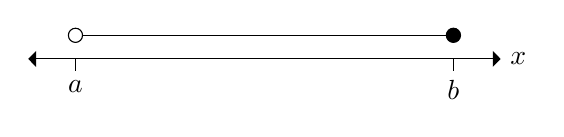
\begin{tikzpicture}[scale=3]
\draw[black, arrows={-Triangle[angle=90:4pt,black,fill=black]}]  (0,0) -- (-1,0);
\draw[black, arrows={-Triangle[angle=90:4pt,black,fill=black]}]  (0,0) -- (1,0) node[anchor=west]{$x$};
\draw (0.8,0.1) -- (-0.8,0.1);
\draw (-0.8,0) -- (-0.8,-0.05) node[anchor=north]{$a$};
\draw (0.8,0) -- (0.8,-0.05) node[anchor=north]{$b$};
\filldraw[fill=white, draw=black] (-0.8,0.1) circle (0.03);
\filldraw[fill=black, draw=black] (0.8,0.1) circle (0.03);
\end{tikzpicture}
\end{center}
	\1 Rules for solving inequalities
		\2 With inequalities, they follow similar rules to solving linear equations, except for two important rules. When multiplying or dividing by a negative number one must reverse the inequality sign. If the sides are switched, one must also reverse the inequality sign.
	\1 Solving inequalities
		\2 When solving inequalities, unless multiplying or dividing by a negative or switching the sides, one must treat the inequality sign as if it is an equals sign. This means that when an operation is completed on one side, the same operation must be completed on the other side.
			\3 Examples
				\[\text{Example One: }3x + 4 > 13\]
				\[3x > 9\]
				\[\therefore x > 3\]
				
				\[\text{Example Two: }4-\frac{x}{3}\leq 6\]
				\[-\frac{x}{3}\leq 2\]
				\[\therefore x \geq -6\]

\0
\subsection{Graphing straight lines}
	\1 Definitions
		\2 The gradient, $m$, is a number that describes the slope of a line. A zero gradient is horizontal, an infinite gradient is vertical. A positive gradient goes upwards from $x$ negative to $x$ positive, while a negative gradient goes downwards from $x$ negative to $x$ positive.
			\[gradient = m = \frac{rise}{run}\]
		\2 The intercepts are the points where the line crosses the $x$-axis and the $y$-axis.
			\3 The $y$-intercept is where $x$ = 0.
			\3 The $x$-intercept is where $y$ = 0.
	\1 Special lines
		\2 Special lines include those with only one axis intercept, and those with their two axis intercepts both at the origin.
			\3 horizontal lines $y = c$ where c is the $y$-intercept
			\3 vertical lines $x = k$ where k is the $x$-intercept
			\3 lines passing through the origin $y = mx$
	\1 Common forms of straight line (linear) equations
		\2 The gradient-intercept form of a straight line is $y = mx + c$ where $m$ is the gradient and $c$ is the $y$-coordinate of the $y$-intercept.
		\2 In two dimensions, straight line graphs can be represented with linear equations. The common forms of linear equations are $y = mx+c$ and $ax+by=d$ where $a, b, c, d$ and $m$ are constants. From linear equations graphs can be drawn.
			\3 Examples
			\3 Shown is $y = -2$, $x = -2$, and $y = \frac{1}{2}x$
\begin{center}
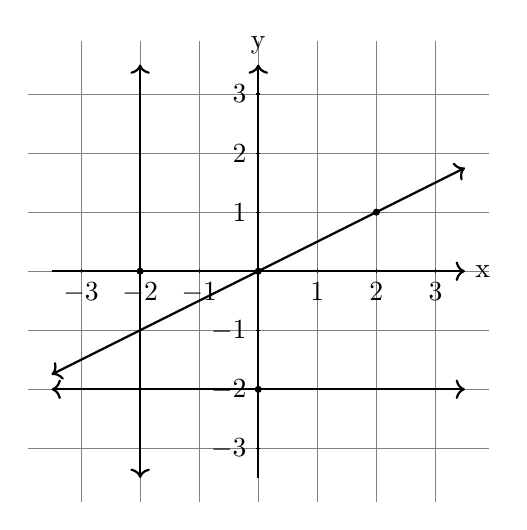
\begin{tikzpicture}[scale=0.75]
\draw[step=1cm,gray,very thin] (-3.9,-3.9) grid (3.9,3.9);
\foreach \x in {-3,-2,-1,1,2,3}
	\draw (\x cm,1pt) -- (\x cm,-1pt) node[anchor=north] {$\x$};
\foreach \y in {-3,-2,-1,1,2,3}
	\draw (1pt,\y cm) -- (-1pt,\y cm) node[anchor=east] {$\y$};
\draw[thick,->] (-3.5,0) -- (3.5,0) node[anchor=west] {x};
\draw[thick,->] (0,-3.5) -- (0,3.5) node[anchor=south] {y};
\draw[thick,<->] (-2,-3.5) -- (-2,3.5);
\draw[thick,<->] (-3.5,-2) -- (3.5,-2);
\draw[thick,<->] (-3.5,-1.75) -- (3.5,1.75);
\filldraw[fill=black, draw=black] (-2,0) circle (0.05);
\filldraw[fill=black, draw=black] (0,-2) circle (0.05);
\filldraw[fill=black, draw=black] (2,1) circle (0.05);
\filldraw[fill=black, draw=black] (0,0) circle (0.05);
\end{tikzpicture}
\end{center}
	\1 Deciding if a point is on a line
		\2 In the form $y = mx + c$, one must substitute the $x$ and $y$ coordinates of the point into the equation. If the equation is equal, the point must be on the line.
			\3 Examples -- Using the point $(-2, 7)$
				\[\text{Example One: }y = -3x + 1\]
				\[7 = -3(-2) + 1\]
				\[7 = 7\]
				\[\therefore (-2,7) \text{ is on the line.}\]
				
				\[\text{Example Two: }2x+2y=1\]
				\[2(-2) + 2(7) = 1\]
				\[-4 + 14 = 1\]
				\[10 \ne 1\]
				\[\therefore (-2, 7) \text{ is not on the line.}\]
	\1 Finding $x$- and $y$-intercepts from linear equations
		\2 To find the $x$-intercept, one needs to substitute $y$ with $0$, as the $x$-intercept is at $y=0$. Once $0$ is substituted in, solving the equation will find the $x$-intercept. To find the $y$-intercept, the reverse is necessary. One must substitute $x$ with $0$, as the $y$-intercept is at $x=0$. Once one has substituted $0$ in, solving the equation will yield the $y$-intercept.
			\3 Examples
				\[\text{Example One: }y = 2x - 8\]
				\[y\text{-intercept } (x=0):\]
				\[y = 2(0) - 8\]
				\[y = -8\]
				\[\text{The }y\text{-intercept is }{-8}\]
				\[x\text{-intercept } (y=0):\]
				\[0 = 2x - 8\]
				\[8 = 2x\]
				\[x = 4\]
				\[\text{The }x\text{-intercept is }4\]
				
				\[\text{Example Two: }-3x - 2y = 6\]
				\[y\text{-intercept }(x=0):\]
				\[-3(0) - 2y = 6\]
				\[-2y = 6\]
				\[y = -3\]
				\[\text{The }y\text{-intercept is }{-3}\]
				\[x\text{-intercept } (y=0):\]
				\[-3x - 2(0) = 6\]
				\[-3x = 6\]
				\[x = -2\]
				\[\text{The }x\text{-intercept is }{-2}\]

\0
\subsection{Finding a rule for a linear graph}
	\1 Finding the gradient of a line
		\2 To determine the gradient of a line, one must have the coordinates of two points. Preferably one of the points is the $y$-intercept, but this is only necessary if one wants to find the rule and not just the gradient. The rule to find the gradient is the difference between two $y$-coordinates ``$y_2$'' and ``$y_1$'', divided by the difference between two $x$-coordinates ``$x_2$'' and ``$x_1$''.
			\3 Equation
				\[m = \frac{y_2 - y_1}{x_2 - x_1}\]
				\[\text{where }(x_1, y_1)\text{ and }(x_2, y_2)\text{ are points on the line}\]
				
	\1 Finding the equation of a line given the $y$-intercept and a point.
		\2 Using the $y$-intercept and a point, one can find the equation of a line. Using the $m = \frac{y_2 - y_1}{x_2 - x_1}$ equation where $(x_1, y_1)$ is the $x$-intercept, one can easily substitute $x_1$ as $c$ in the equation $y = mx + c$. With $m$ and $c$ constructed, one is able to construct a full equation.
			\3 Equation
				\[y = \left(\frac{y_2 - y_1}{x_2 - x_1}\right)x + (y_1)\]
 
\0
\subsection{Length and midpoint of a line segment}
	\1 Length of a line segment
		\2 The length of a line segment is found using a variant of the Pythagoras' theorem. It involves finding the difference between $y_2$ and $y_1$, and $x_2$ and $x_1$, squaring them individually, adding them together, and then performing a square root on the sum.
			\3 Equation
				\[d = \sqrt{(x_2 - x_1)^2 + (y_2 - y_1)^2}\]
				
	\1 Midpoint of a line segment
		\2 The midpoint of a line segment, known as $M$, is the point exactly halfway in between two points $(x_1, y_1)$ and $(x_2, y_2)$.
			\3 Equation
				\[M = \left(\frac{x_1 + x_2}{2}, \frac{y_1 + y_2}{2}\right)\]

\0
\subsection{Perpendicular and parallel lines}
	\1 Parallel Postulate
		\2 ``It is true that if a straight line falling on two straight lines makes the interior angles on the same side less than two right angles, the two straight lines, if produced indefinitely, intersect on that side on which are the angles less than the two right angles.'' --Euclid of Alexandria
	\1 Explanation
		\2 If a straight line is placed in a perpendicular position across two lines, and the cointerior angles do not sum to 180\degree, the two lines are not parallel.
	\1 How to determine parallel and perpendicular lines
		\2 Two parallel lines have the same gradient. Two perpendicular lines with gradients $m_1$ and $m_2$ will adhere to the following rules (it is not necessary to test both):
			\[m_1 \times m_2 = -1\]
			\[m_2 = -\frac{1}{m_1}\]

\0
\subsection{Simultaneous equations - substitution}
	\1 What are simultaneous equations
		\2 Simultaneous equations are a set of equations, where the goal is generally to find the point where the graphs of the two equations meet. The two equations must be non-parallel, as there is no point of intersection in a set of parallel equations.
	\1 Substitution
		\2 Solving a simultaneous equation can be done in two ways. Using the substitution method is usually due to at least one of the equations having one variable as the subject. The substitution method involves substituting one equation into the other, followed by solving the equation to yield the other variable. That variable can be substituted back into the equation, to solve the first variable.
			\3 Examples
%WATCH THE FORMATTING HERE - SPACES ARE KINDA SCREWY
				\[(1)\ \ \ \ \ \ \ \ y = 3x + 2\]
				\[(2)\ \ \ \ \ \ \ \ y = 7x - 8\]
				\[\text{Substitute equation (2) into equation (1)}\]
				\[7x - 8 = -3x + 2\]
				\[10x = 10\]
				\[x = 1\]
				\[\text{Substitute $x = 1$ into equation (1)}\]
				\[y = -3(1) + 2\]
				\[y = -1\]
				\[\text{Solution is }(1, -1)\]
				
\0
\subsection{Simultaneous equations - elimination}
	\1 What are simultaneous equations
		\2 Simultaneous equations are a set of equations, where the goal is generally to find the point where the graphs of the two equations meet. The two equations must be non-parallel, as there is no point of intersection in a set of parallel equations.
	\1 Elimination
		\2 The method of elimination as a way of solving simultaneous equations is often used when both equations are in the form of $ax + by = d$. The elimination method involves adding or subtracting two equations to eliminate one of the two variables in the result. If there are no ways to eliminate them, often multiplying one can help in eliminating the variable in question.
			\3 Examples
%WATCH THE FORMATTING HERE - SPACES ARE KINDA SCREWY
				\[(1)\ \ \ \ \ \ \ \ y - 3x = 1\ \ \ \]
				\[(2)\ \ \ \ \ \ \ \ 2y - 5x = 13\]
				\[(1)\times2 => (3)\ \ \ \ \ \ \ \ 2y - 6x = 2\ \ \ \ \ \ \ \ \ \ \ \ \ \ \ \ \ \]
				\[(2)-(3)\ \ \ \ \ \ \ \ 11x = 11\ \ \ \ \ \ \ \ \ \ \ \ \]
				\[\ \ \ x = 1\]
				\[\ \ \ \ \ \ \ \ \ \ \ \ \text{Substitute $x = 1$ into equation (1)}\]
				\[\ \ \ \ \ \ \ \ \ \ \ \ \ y - 3(1) = 1\]
				\[\ \therefore y = 4\]
				\[\text{Solution is }(1,4)\ \ \ \ \ \ \ \ \ \ \ \]
				
\0
\subsection{Further applications of simultaneous equations}
	\1 Setting up and solving simultaneous equations
		\2 Setting up a simultaneous equation is the process of finding two solvable equations from text. One must define a variable for each unknown, write down two equations from the information given, solve the equations simultaneously to find the solution, and interpret the solution and answer the question in words.
			\3 Example
%WATCH THE FORMATTING HERE - SPACES ARE KINDA SCREWY

				The sum of the ages of two children is 17 and the difference in their ages is 5. If Kara is the older sister of Ben, determine their ages.
				
				\[\text{Let $k$ be Kara's age and $b$ be Ben's age}\]
				\[(1)\ \ \ \ \ \ \ \ k + b = 17\]
				\[(2)\ \ \ \ \ \ \ \ k - b = 5\ \]
				\[\ \ (1)+(2)\ \ \ \ \ \ \ \ 2k = 22\ \ \ \ \ \ \ \ \ \ \ \ \]
				\[\ \ \ \ \ \therefore k = 11\]
				\[\text{Substitute } k = 11 \text{ into equation } (1)\]
				\[\ \ \ \ \ \ \ \ \ \ \ \ \ \ 11 + b = 17\]
				\[\ \ \ \ \therefore b = 5\]
	\1 Solving further applications with two variables
		\2 To solve further applications with two variables, the elimination method of solving simultaneous equations is ideal to use.
			\3 Example
%WATCH THE FORMATTING HERE - SPACES ARE KINDA SCREWY

				John buys 3 daffodils and 5 petunias from the nursery and pays \$25. Julia buys 4 daffodils and 3 petunias for \$26. Determine the cost of each type of flower.
				
				\[\text{Let \$$d$ be the cost of a daffodil and \$$p$ be the cost of a petunia}\]
				\[\]
				\[(1)\ \ \ \ \ \ \ \ 3d + 5p = 25\ \]
				\[(2)\ \ \ \ \ \ \ \ 4d + 3p = 26\ \]
				\[(1)\times4 => (3)\ \ \ \ \ \ \ \ 12d + 20p = 100\ \ \ \ \ \ \ \ \ \ \ \ \]
				\[(2)\times3 => (4)\ \ \ \ \ \ \ \ 12d + 9p = 78\ \ \ \ \ \ \ \ \ \ \ \ \ \ \ \]
				\[(3) - 4 =>\ \ \ \ \ \ \ \ 11p = 22\ \ \ \ \ \ \ \ \ \ \ \ \ \ \ \ \ \]
				\[\therefore p = 2\]

\0
\subsection{Half planes}
	\1 Linear equalities
		\2 A linear inequality with one variable can be solved using the same method as solving an inequality.
		\2 The solution to a linear inequality with two variables is illustrated using a half plane.
		\2 If the equation is of the form $ax + by = d$, it is usually simpler to test a point to see which side of the line is included in the region.
		\2 If $y$ is the subject of the inequality follow these simple rules:
			\3 $y \geq mx + c$
				\4 Draw a solid line (as it is included in the region) and shade above.
			\3 $y > mx + c$
				\4 Draw a broken line (as it is included in the region) and shade above.
			\3 $y \leq mx + c$
				\4 Draw a solid line (as it is included in the region) and shade below.
			\3 $y < mx + c$
				\4 Draw a broken line (as it is included in the region) and shade below.
		\2 Examples
\begin{center}
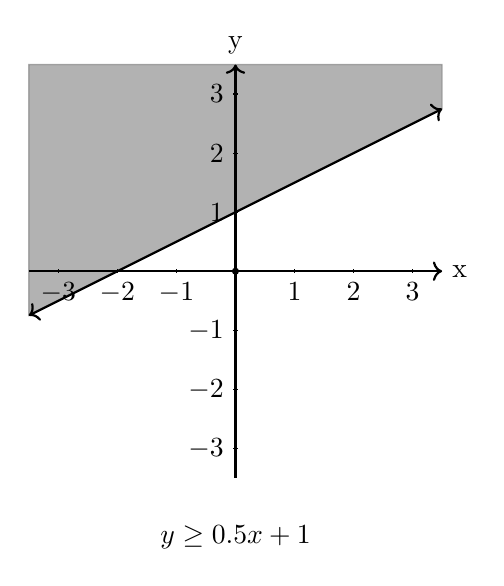
\begin{tikzpicture}[scale=0.75]
\filldraw[fill=black, opacity=0.3] (-3.5,-0.75) -- (3.5,2.75) -- (3.5,3.5) -- (-3.5,3.5) -- cycle;
\foreach \x in {-3,-2,-1,1,2,3}
	\draw (\x cm,1pt) -- (\x cm,-1pt) node[anchor=north] {$\x$};
\foreach \y in {-3,-2,-1,1,2,3}
	\draw (1pt,\y cm) -- (-1pt,\y cm) node[anchor=east] {$\y$};
\draw[thick,->] (-3.5,0) -- (3.5,0) node[anchor=west] {x};
\draw[thick,->] (0,-3.5) -- (0,3.5) node[anchor=south] {y};
\draw[thick,<->] (-3.5,-0.75) -- (3.5,2.75);
\filldraw[fill=black, draw=black] (0,0) circle (0.05);
\node at (0, -4.5){$y \geq 0.5x + 1$};
\end{tikzpicture}
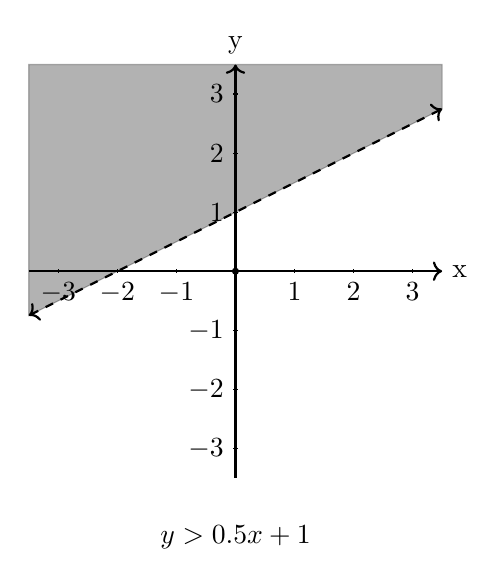
\begin{tikzpicture}[scale=0.75]
\filldraw[fill=black, opacity=0.3] (-3.5,-0.75) -- (3.5,2.75) -- (3.5,3.5) -- (-3.5,3.5) -- cycle;
\foreach \x in {-3,-2,-1,1,2,3}
	\draw (\x cm,1pt) -- (\x cm,-1pt) node[anchor=north] {$\x$};
\foreach \y in {-3,-2,-1,1,2,3}
	\draw (1pt,\y cm) -- (-1pt,\y cm) node[anchor=east] {$\y$};
\draw[thick,->] (-3.5,0) -- (3.5,0) node[anchor=west] {x};
\draw[thick,->] (0,-3.5) -- (0,3.5) node[anchor=south] {y};
\draw[thick,<->, dashed] (-3.5,-0.75) -- (3.5,2.75);
\filldraw[fill=black, draw=black] (0,0) circle (0.05);
\node at (0, -4.5){$y > 0.5x + 1$};
\end{tikzpicture}
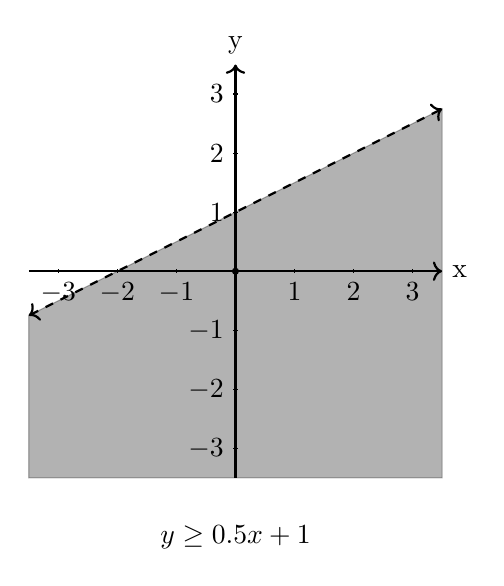
\begin{tikzpicture}[scale=0.75]
\filldraw[fill=black, opacity=0.3] (-3.5,-0.75) -- (3.5,2.75) -- (3.5,-3.5) -- (-3.5,-3.5) -- cycle;
\foreach \x in {-3,-2,-1,1,2,3}
	\draw (\x cm,1pt) -- (\x cm,-1pt) node[anchor=north] {$\x$};
\foreach \y in {-3,-2,-1,1,2,3}
	\draw (1pt,\y cm) -- (-1pt,\y cm) node[anchor=east] {$\y$};
\draw[thick,->] (-3.5,0) -- (3.5,0) node[anchor=west] {x};
\draw[thick,->] (0,-3.5) -- (0,3.5) node[anchor=south] {y};
\draw[thick,<->, dashed] (-3.5,-0.75) -- (3.5,2.75);
\filldraw[fill=black, draw=black] (0,0) circle (0.05);
\node at (0, -4.5){$y \geq 0.5x + 1$};
\end{tikzpicture}
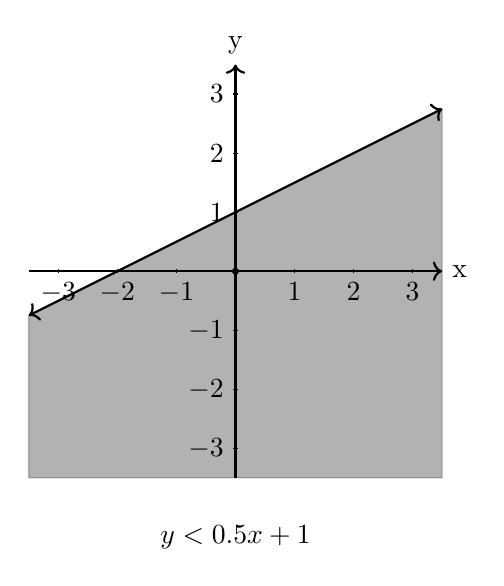
\begin{tikzpicture}[scale=0.75]
\filldraw[fill=black, opacity=0.3] (-3.5,-0.75) -- (3.5,2.75) -- (3.5,-3.5) -- (-3.5,-3.5) -- cycle;
\foreach \x in {-3,-2,-1,1,2,3}
	\draw (\x cm,1pt) -- (\x cm,-1pt) node[anchor=north] {$\x$};
\foreach \y in {-3,-2,-1,1,2,3}
	\draw (1pt,\y cm) -- (-1pt,\y cm) node[anchor=east] {$\y$};
\draw[thick,->] (-3.5,0) -- (3.5,0) node[anchor=west] {x};
\draw[thick,->] (0,-3.5) -- (0,3.5) node[anchor=south] {y};
\draw[thick,<->] (-3.5,-0.75) -- (3.5,2.75);
\filldraw[fill=black, draw=black] (0,0) circle (0.05);
\node at (0, -4.5){$y < 0.5x + 1$};
\end{tikzpicture}
\end{center}

	\1 Sketching half planes
		\2 To sketch a half plane, one must find the $x$- and $y$- intercepts, and mark them on a graph. From there, one is able to draw the complete line of the graph. If the $x$- and $y$- intercepts are both at zero, one must substitute in a value other than 0 into the $x$ or $y$ co-efficient, and calculate the equation. The result, combined with the 
	\1 Finding the intersecting region

\end{outline}

\newpage

\section{Geometry}
\begin{outline}

\0
\subsection{Geometry reiterated}

\0
\subsection{Congruent triangles}

\0
\subsection{Investigating parallelograms using congruence}

\0
\subsection{Similar figures}

\0
\subsection{Proving similar triangles}

\0
\subsection{Circles and chord properties}

\0
\subsection{Angle properties of circles - theorems 1 and 2}

\0
\subsection{Angle properties of circles - theorems 3 and 4}

\0
\subsection{Tangents}

\0
\subsection{Intersecting chords, secants, and tangents}
\end{outline}

\newpage

\section{Indices and Surds}
\begin{outline}

\0
\subsection{Irrational numbers and surds}
	\1 Square factors
		\2 When a factor of a number is a perfect square it can be called a square factor.
			\3 Examples of square numbers
				\[4,\ 9,\ 16,\ 25,\ 36,\ 49,\ 64,\ 81,\ 100\dots\]
	\1 Real numbers
		\2 Real numbers are numbers that can be located on a number line as a point. They include rational numbers, which are numbers able to be represented as fractions. The decimal form of a rational number either ends in recurring digits or ends by way of termination. Rational numbers take the form of either fractions or decimals. Irrational numbers, are numbers that cannot be expressed as fractions. The decimal representation of an irrational number is an infinite non-recurring decimal. Irrational numbers cannot be expressed in the form $\frac{a}{b}$ where $a$ and $b$ are integers and $b \ne 0$.
			\3 Rational numbers
				\[\frac{3}{7}, {-\frac{4}{39}}, -3, 1.6, 2.\dot7, 0.\overline{19}\]
			\3 Irrational numbers
				\[\sqrt{3}, {-2}\sqrt{7}, \sqrt{12} - 1, \pi, 2\pi - 3\]
	\1 Surds
		\2 Surds are irrational numbers that use a root sign.
			\3 These are surds:
				\[\sqrt{2}, \sqrt[5]11, {-\sqrt{200}}, 1 + \sqrt{5}\]
			\3 These are not surds:
				\[\sqrt{4}\ (=2), \sqrt[3]{125}\ (=5), -\sqrt[4]{16}\ (=-4)\]
	\1 Rules that apply to surds
		\[(\sqrt{x})^2 = x \text{\ and\ } \sqrt{x^2} = x \text{\ \ \ \ if\ \ \ \ } x \geq 0\]
		\[\sqrt{xy} = \sqrt{x} \times \sqrt{y} \text{\ \ \ \ if\ \ \ \ } x \geq 0 \text{\ and\ } y \geq 0\]
		\[\sqrt{\frac{x}{y}} = \frac{\sqrt{x}}{\sqrt{y}} \text{\ \ \ \ if\ \ \ \ } x \geq 0 \text{\ and\ } y > 0\]
	\1 Deciding if a number is rational or irrational
		\2 The method for finding whether a number is rational or irrational involves expressing the number as a decimal. If there is no recurring pattern, and the decimal doesn't terminate, one is dealing with an irrational number. If either of those conditions aren't followed, the number must be rational, and therefore not a surd.
	\1 Simplifying surds
		\2 To simplify a surd, one must identify what type of surd they are trying to simplify. There are four common types of surds, all which are simplified using different methods.
			\3 $\sqrt{x}$ surd - simplified by splitting the radicand into the highest square factor and the other factor the radicand divides into. This can then be split into two square roots - one which is a surd, and one which can be simplified. After simplifying the second square root, the expression can be shown as $y\sqrt{x}$ where $x$ is the surd and $y$ is the simplified square root. This is not to be confused with $\sqrt[y]{x}$, which denotes the $y$-th root of $x$ instead of $y$ multiplied by the square root of {x}.
				\[\sqrt{32} = \sqrt{16 \times 2}\]
				\[= \sqrt{16} \times \sqrt{2}\]
				\[= 4\sqrt{2}\]
			\3 $y\sqrt{x}$ surd - simplified by splitting the radicand into the highest square factor and the other factor the radicand divides into. This can then be split into two square roots - one which is a surd, and one which can be simplified. After simplifying the second square root, the two numbers not in root form can be multiplied together to make the final form a simplified $y\sqrt{x}$.
				\[3\sqrt{200} = 3\sqrt{100 \times 2}\]
				\[= 3 \times \sqrt{100} \times \sqrt{2}\]
				\[= 3 \times 10 \times \sqrt{2} = 30\sqrt{2}\]
			\3 $\frac{y\sqrt{x}}{z}$ surd - simplified by splitting the radicand into the highest square factor and the other factor the radicand divides into. This can then be split into two square roots - one which is a surd, and one which can be simplified. After simplifying the second square root, the two numbers not in root form (in the numerator) can be multiplied together. If there are any factors that can be cancelled in the final expression, they must be cancelled to make the expression the simplest form.
				\[\frac{5\sqrt{40}}{6} = \frac{5\sqrt{4\times 10}}{6}\]
				\[= \frac{5 \times \sqrt{4} \times \sqrt{10}}{6}\]
				\[= \frac{\cancelto{5}{10} \sqrt{10}}{\cancelto{3}{6}}\]
				\[= \frac{5\sqrt{10}}{3}\]
			\3 The last common form of surd is trivial to solve by removing the fraction's root and applying the root to both the numerator and denominator. From there, the normal method of solving fraction-based surds can be used.
				\[\sqrt{\frac{x}{y}} = \frac{\sqrt{x}}{\sqrt{y}}\]
	\1 Expressing surds as a square root of a positive integer (entire surds)
		\2 To express surds as a square root of a positive integer, one must express the $y$ of $y\sqrt{x}$ as the square root of the square of y. Then the two square roots can be combined.
			\[2\sqrt{5} = \sqrt{4} \times \sqrt{5} = \sqrt{20}\]

\0
\subsection{Adding and subtracting surds}
	\1 Like surds
	 	\2 Like surds are multiples of the same surd. Like surds can be added and subtracted. Before attempting to add or subtract surds, one must simplify all surds.
	 	 	\3 Examples
	 	 	 	\[\sqrt{3}, -5\sqrt{3}, \sqrt{12} (= 2\sqrt{3}), 2\sqrt{75} (= 10\sqrt{3})\]
	\1 Adding or subtracting surds using like terms.
	 	\2 Adding and subtracting surds is very simple. It involves making the $\sqrt{x}$ in the $y\sqrt{x}$ surd form (where $y$ is either implied to be 1, or is represented by a different number) equal in each term one wants to add or subtract, then combining the $y$ by either addition or subtraction, while keeping $\sqrt{x}$ the same.
	 	 	\3 Examples
	 	 	 	\[2\sqrt{3} + 4\sqrt{3}\]
	 	 	 	\[= 6\sqrt{3}\]
	 	 	 	\[\]
	 	 	 	\[9\sqrt{5} - 4\sqrt{5}\]
	 	 	 	\[= 5\sqrt{5}\]
	\1 Simplifying surds in order to add or subtract
	 	\2 Surds must be simplified to have the same radicand and index before they can be added or subtracted. To do this, one must identify the type of surd they are dealing with, and follow the correct steps to change the form of the surd. \textit{Refer to ``Irrational numbers and surds'' for more information on simplifying surds.}

\0
\subsection{Multiplying and dividing surds}
	\1 Rules for multiplying and dividing surds
	 	\2 When multiplying surds, the result will, in most common situations, abide by these rules:
	 	 	\[\sqrt{x} \times \sqrt{y} = \sqrt{xy}\]
	 	 	\[\text{Generally: } a\sqrt{x} \times b\sqrt{y} = ab\sqrt{xy}\]
	 	\2 When dividing surds, the result will, in most common situations, abide by these rules:
	 	 	\[\frac{\sqrt{x}}{\sqrt{y}} = \sqrt{\frac{x}{y}}\]
	 	 	\[\text{Generally: } \frac{a\sqrt{x}}{b\sqrt{y}} = \frac{a}{b}\sqrt{\frac{x}{y}}\]
	 	\2 When expanding brackets, the distributive law applies to surds as much as any other algebra:
	 	 	\[a(b+c) = ab+ac\]
	\1 Simplifying a product of two surds
	 	\2 To simplify the product of two surds, one must utilise the rules for multiplying surds.
	 	 	\3 Examples
	 	 	 	\[\sqrt{2} \times \sqrt{3}\]
	 	 	 	\[= \sqrt{2 \times 3}\]
	 	 	 	\[= \sqrt{6}\]
	 	 	 	\[\]
	 	 	 	\[2\sqrt{3} \times 3\sqrt{15}\]
	 	 	 	\[= 2 \times 3 \times \sqrt{3 \times 15}\]
	 	 	 	\[= 6\sqrt{45}\]
	 	 	 	\[= 6\sqrt{9 \times 5}\]
	 	 	 	\[= 18\sqrt{5}\]
	\1 Simplifying surds using division
	 	\2 To simplify surds using division, one must utilise the rules for dividing surds.
	 	 	\3 Examples
	 	 	 	\[-\sqrt{10} \div \sqrt{2}\]
	 	 	 	\[= -\sqrt{\frac{10}{2}}\]
	 	 	 	\[= -\sqrt{5}\]
	 	 	 	\[\]
	 	 	 	\[\frac{12\sqrt{18}}{3\sqrt{3}}\]
	 	 	 	\[= \frac{12}{3}\sqrt{\frac{18}{3}}\]
	 	 	 	\[= 4\sqrt{6}\]
	\1 Using the distributive law
	 	\2 To use the distributive law, one must multiply the external multiplier by each term within the brackets.
	 		\3 Examples
	 			\[\sqrt{3}(3\sqrt{5}-\sqrt{6})\]
	 			\[= 3\sqrt{15}-\sqrt{18}\]
	 			\[= 3\sqrt{15}-\sqrt{9 \times 2}\]
	 			\[= 3\sqrt{15}-3\sqrt{2}\]
	 			\[\]
	 			\[-3\sqrt{6}(2\sqrt{10}-4\sqrt{6})\]
	 			\[= -6\sqrt{60}+12\sqrt{36}\]
	 			\[= -6\sqrt{4 \times 15}+12 \times 6\]
	 			\[= -12\sqrt{15}+72\]

\0
\subsection{Binomial products}
	\1 Expanding binomial products
		\2 To expand binomial products, one must use the distributive law. This says that the first, outer, inner, and last pairs ``F.O.I.L.'' multiplied individually, then added together is equal to the binomial product.
			\3 F.O.I.L
				\[\text{First: }(\textbf{a} + b)(\textbf{c} + d)\]
				\[\text{Outer: }(\textbf{a} + b)(c + \textbf{d})\]
				\[\text{Inner: }(a + \textbf{b})(\textbf{c} + d)\]
				\[\text{Last: }(a + \textbf{b})(c + \textbf{d})\]
			\3 Equation
				\[(a + b)(c + d) = ac + ad + bc + bd\]

			\3 Examples
				\[(4 + \sqrt{3})(\sqrt{3} - 2)\]
				\[= 4\sqrt{3} - 8 + 3 - 2\sqrt{3}\]
				\[= 2\sqrt{3} - 5\]
				\[\]
				\[(2\sqrt{5} - 1)(3\sqrt{5} + 4)\]
				\[= 6 \times 5 + 8\sqrt{5} - 3\sqrt{5} - 4\]
				\[= 30 + 5\sqrt{5} - 4\]
				\[= 26 + 5\sqrt{5}\]
	\1 Expanding perfect squares
		\2 Expanding perfect squares is done by removing the square, and representing the equation as a binomial product.  If the equation has a negative before expanding, in the form $(x - y)^2$, From there, the problem may be solved through the normal process of expanding binomial products.
			\[(x + y)^2 = (x + y)(x + y)\]
	 	 	\[(x - y)^2 -(x + y)(x - y)\]
 	 	 	\[\]
 	 	 	\[(a + b)^2\]
 	 	 	\[a^2 + ab + ba + b^2\]
	 	 	\[a^2 + 2ab + b^2\]
	 	 	\[\]
	 	 	\[(a - b)^2\]
	 	 	\[a^2 - ab - ba + b^2\]
	 	 	\[a^2 - 2ab + b^2\]

\0
\subsection{Rationalising the denominator}
	\1 Method of rationalising a denominator
		\2 Rationalising a denominator is to change the denominator of a surd to a rational number. This is achieved by multiplying by a number equivalent to 1. The number equivalent to 1 will almost always be the radical and radicand within the denominator over the radical and radicand within the denominator. As $\frac{x}{x}$ = 1, this will always be equivalent to 1.
			\3 Method
				\[\frac{x}{\sqrt{y}} = \frac{x}{\sqrt{y}} \times \frac{\sqrt{y}}{\sqrt{y}} = \frac{x\sqrt{y}}{y}\]
			\3 Examples
				\[\frac{2}{\sqrt{3}} = \frac{2}{\sqrt{3}} \times \frac{\sqrt{3}}{\sqrt{3}} = \frac{2\sqrt{3}}{3}\]

\0
\subsection{Index laws reiterated}
	\1 Index laws
		\2 The first law
			\[a^m \times a^n = a^{m+n}\]
		\2 The second law
			\[a^m \div a^n = \frac{a^m}{a^n} = a^{m-n}\]
		\2 The third law
			\[(a^m) ^n = a^{m \times n}\]
		\2 The fourth law
			\[(a \times b)^m = a^m \times b^m\]
		\2 The fifth law
			\[\left(\frac{a}{b}\right)^m = \frac{a^m}{b^m}\]
		\2 Zero powers
			\[a^0 = 1\]
	\1 Using the first law
		\2 The first index law allows one to multiply expressions with indices, by retaining the base, and adding together the indices.
			\3 Examples
				\[x^5 \times x^4 = x^9\]
				\[3a^2b \times 4ab^3 = 12a^3b^4\]
	\1 Using the second law
		\2 The second index law states the method for dividing expressions with indices is to retain the base, and subtract the indices.
			\3 Examples
				\[m^7 \div m^5 = m^2\]
				\[4x^2y^5 \div (8xy^2) = \frac{4}{8}xy^3 = \frac{1}{2}xy^3\]
	\1 Using the third law
		\2 The third index law describes the method for expanding expressions with parenthetical indices, where the parentheses contain a term with an index, through retaining the base and multiplying the indices.
			\3 Examples
				\[(x^3)^6 = x^{18}\]
				\[(3x^4)^4 = 81x^{16}\]
	\1 Using the fourth law
		\2 The fourth index law describes the method for expanding parenthesis with an exterior index, by distributing the index number across the bases.
			\3 Examples
				\[(6 \times 9)^3 = 6^3 \times 9^3\]
				\[(4x \times 3y)^4 = 4x^4 \times 3y^4\]
	\1 Using the fifth law
		\2 The fifth index law enables simplification and rearrangement of fractions within parenthesis where there is an exterior index.
			\3 Examples
				\[\left(\frac{3x}{2y}\right)^3 = \frac{3x^3}{2y^3}\]
				\[\left(\frac{3xy}{2}\right)^5 = \frac{243x^5y^5}{32}\]

\0
\subsection{Negative indices}
	\1 Rules of negative indices
		\[a^{-m} = \frac{1}{a^m}\]
		\[\frac{1}{a^{-m}} = a^m\]
	\1 Writing expressions using positive indices
		\2 To write an expression with negative indices in a form that uses positive indices, one must use the rules of negative indices, combined with the index laws where necessary.
			\3 Examples
				\[b^{-4} = \frac{1}{b^4}\]
				\[3x^{-4}y^2 = \frac{3y^2}{x^4}\]

\0
\subsection{Scientific notation}
	\1 Rules of scientific notation
		\2 A number written using scientific notation is of the form $a \times 10^m$ where $1 \leq a < 10$ and $m$ is an integer.
		\2 Significant figures are the number of digits counted from left to right, starting at the first non-zero. Significant figures are a useful measure of decimal point accuracy using scientific notation.
			\3 Examples
				\[2.019 \times 10^7 \text{ has 4 significant figures.}\]
				\[3.44426 \times 10^3 \text{ has 6 significant figures.}\]
	\1 Converting from scientific notation to a basic numeral
		\2 To convert from scientific notation to basic numerals, one must move the decimal point. The direction and degree to which the decimal point must be moved is dependent on the index, $m$, in $a \times 10^m$. If the index is positive, the decimal point must be moved to the right. Conversely, if the index is negative, the decimal point must be moved to the left. The index itself represents the number of places the decimal point must be moved.
			\3 Examples
				\[5.016 \times 10^5 = 501600\]
				\[3.2 \times 10^{-7} = 0.00000032\]
	\1 Converting from basic numerals to scientific notation
		\2 To convert from basic numerals to scientific notation, one must move the decimal point (in the reverse direction than converting from scientific notation to basic numerals), then add the notation that specifies the exponent and multiplier. First, one must choose the number of places to move the decimal point. As scientific notation specifies that the number be less than 10 and equal or greater than 1, this number can be found by counting the number of places between the current position and the position after the first non-zero digit. This number, which will be positive if counting towards the left, or negative if counting toward the right, will become the index, $m$, in $a \times 10^m$.
			\3 Examples
				\4 3 significant figures
					\[5218300 = 5.22 \times 10^6\]
					\[0.0042031 = 4.20 \times 10^{-3}\]
				\4 6 significant figures
					\[225502849 = 2.25503 \times 10^8\]
					\[0.0008456832 = 8.45683 \times 10^{-4}\]

\0
\subsection{Rational indices}
	 \1 Rules of rational indices
		\[a^{\frac{1}{n}} = \sqrt[n]{a}\]
		\[a^{\frac{m}{n}} = (\sqrt[n]{a})^m\]
	 	\2 Writing in index form
		 	 \3 To write a surd in index form, one must identify the rules of rational indices. Recalling that $a = a^1$, one can change $\sqrt[n]{a^m}$, where $n$ is the index, $a$ is the radicand, and $m$ represents the index of $a$, into $a^{\frac{m}{n}}$.
		 	 	 \4 Examples
	 	 	 	 	 \[\sqrt{15} = 15^{\frac{1}{2}}\]
	 	 	 	 	 \[\sqrt{7x^5} = 7^{\frac{1}{2}}x^{\frac{5}{2}}\]
	 	 	 	 	 \[3\sqrt[4]{x^7} = 3x^{\frac{7}{4}}\]
	 	 	 	 	 \[10\sqrt{10} = 10^{\frac{3}{2}}\]
	 	\2 Writing in surd form
	 	 	\3 To write a number in index form in surd form, one must identify the rules of rational indices. Using the fact that $a = a^1$, one can change a number in index form $a^{\frac{m}{n}}$, where $a$ would become the radicand, $m$ would become the index of $a$, and $n$ would become the index, into the form $\sqrt[n]{a^m}$.
	 	 	 	\4 Examples
	 	 	 	 	\[3^{\frac{1}{5}} = \sqrt[5]{3}\]
	 	 	 	 	\[5^{\frac{2}{3}} = \left(\sqrt[3]{5}\right)^2 = \sqrt[3]{25}\]

\0
\subsection{Exponential equations}
	\1 Simple exponential equations
	 	\2 Simple exponential equations take the form $a^x = b$, where $a > 0$ and $a \neq 1$.
	\1 Solving exponential equations
		\2 To solve exponential equations, one must exploit the fact: if $a^x = a^y$ then $x = y$. This allows simple removal of the base to find the unknown index.
			\3 Examples
				\[2^x = 16\]
				\[2^x = 2^4\]
				\[\therefore x = 4\]
				\[\]
				\[3^x = \frac{1}{9}\]
				\[3^x = \frac{1}{3^2}\]
				\[3^x = 3^{-2}\]
				\[\therefore x = -2\]
				\[\]
				\[25^x = 125\]
				\[(5^2)^x = 5^3\]
				\[5^{2x} = 5^3\]
				\[\therefore 2x = 3\]
				\[\therefore x = \frac{3}{2}\]
	\1 Solving exponential equations with a variable on both sides
		\2 To solve an exponential equation with a variable on both side, one must find a way to make the two bases equal, which will in turn allow for the bases to be removed and the unknown index to be found.
			\3 Examples
				\[3^{2x-1} = 27^x\]
				\[3^{2x-1} = (3^3)^x\]
				\[3^{2x - 1} = 3^{3x}\]
				\[\therefore 2x - 1 = 3x\]
				\[\therefore x = -1\]

\0
\subsection{Exponential growth and compound interest}
	\1 Necessary knowledge
		\2 Exponential growth and decay can be modelled by the rule $A = ka^t$, where $A$ is the amount, $k$ is the initial amount and $t$ is the time. If $a > 0$, exponential growth occurs. If $0 < a < 1$, exponential decay occurs.
		\2 For a growth rate of $r\%$ p.a., the base `a' is calculated using $a = 1 + \frac{r}{100}$.
		\2 For a decay rate of $r\%$ p.a., the base `a' is calculated using $a = 1 - \frac{r}{100}$.
	\1 The exponential formula
		\[A = A_0\left(1 \pm \frac{r}{100}\right)^n\]
		\2 $A$ is the amount
		\2 $A_0$ is the initial amount
		\2 $r$ is the rate expressed as a percentage
		\2 $n$ is the time
		\2 $\pm$ depends on whether the calculation is growth (+) or decay (-)
	\1 Compound interest
		\2 Compound interest involves adding any interest earned to the balance at the end of each year or other period. The rule for the investment amount (\$$A$) is given by:
			\[A = A_0\left(1 + \frac{r}{100}\right)^t\]
			\3 $A_0$ is the initial amount
			\3 $r$ is the interest rate expressed as a percentage
			\3 $t$ is the time
	\1 Writing exponential rules
		\2 Compound interest (growth):
		
			\$100000 in savings at a rate of 14\% per annum
			
			\[A = A_0\left(1 + \frac{r}{100}\right)^n\]
			\[A = 100000\left(1 + \frac{14}{100}\right)^n\]
			\[\therefore A = 100000\left(1.14\right)^n\]
		\2 Population decreasing (decay):
		
			City population of 50000 decreasing by 12\% per year
			
			\[P = P_0\left(1 - \frac{r}{100}\right)^n\]
			\[P = 50000\left(1 - \frac{12}{100}\right)^n\]
			\[\therefore P = 50000\left(0.88\right)^n\]
	\1 Applying exponential rules
		\2 Finding the value after $n$ time
			\3 To find the value, $V$, after $n$ time, one must substitute a real value into the place of $n$. The calculation of this equation will yield $A$.
				\4 Examples
					\[\text{Starting Value: } \$145000 \text{; Growth rate: } 9\%\]
					\[\text{Find $V$ if $n = 1$}\]
					\[V = V_0\left(1.09\right)^n\]
					\[V = 145000\left(1.09\right)^1\]
					\[\therefore V = 158050\]
					\[\]
					\[\text{Find $V$ if $n = 3$}\]
					\[V = V_0\left(1.09\right)^n\]
					\[V = 145000\left(1.09\right)^3\]
					\[\therefore V = 187779.21\]

\end{outline}

\newpage

\section{Trigonometry}
\begin{outline}

\0
\subsection{Trigonometric ratios}
	\1 What is trigonometry?
		\2 Trigonometry is the study of the relationship between the angles and side lengths of triangles. It is built upon three ratios: sine, cosine, and tangent. A common mnemonic is SOHCAHTOA, for remembering the trigonometric ratios, with S representing sine, C representing cosine, and T representing tangent. Respectively, O, A, and H mean opposite, adjacent, and hypotenuse.
		
\begin{center}
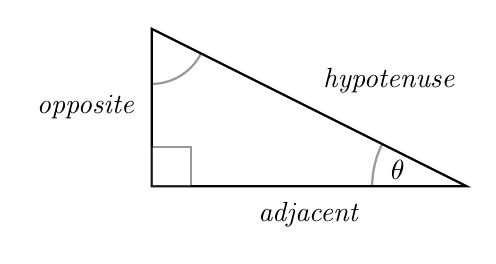
\begin{tikzpicture}[thick]
\coordinate (O) at (0,0);
\coordinate (A) at (4,0);
\coordinate (B) at (0,2);
\draw (O)--(A)--(B)--cycle;

\tkzLabelSegment[below=2pt](O,A){\textit{adjacent}}
\tkzLabelSegment[left=2pt](O,B){\textit{opposite}}
\tkzLabelSegment[above right=2pt](A,B){\textit{hypotenuse}}

\tkzMarkRightAngle[fill=white,size=0.5,opacity=.4](A,O,B)
\tkzLabelAngle[pos = 0.35](A,O,B){}

\tkzMarkAngle[fill= white,size=1.2cm,%
opacity=.4](B,A,O)
\tkzLabelAngle[pos = 0.9](B,A,O){$\theta$}

\tkzMarkAngle[fill= white,size=0.7cm,%
opacity=.4](O,B,A)
\tkzLabelAngle[pos = 0.5](O,B,A){}

\end{tikzpicture}
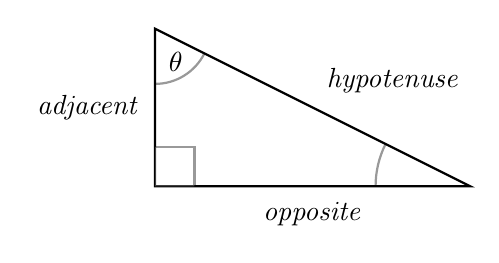
\begin{tikzpicture}[thick]
\coordinate (O) at (0,0);
\coordinate (A) at (4,0);
\coordinate (B) at (0,2);
\draw (O)--(A)--(B)--cycle;

\tkzLabelSegment[below=2pt](O,A){\textit{opposite}}
\tkzLabelSegment[left=2pt](O,B){\textit{adjacent}}
\tkzLabelSegment[above right=2pt](A,B){\textit{hypotenuse}}

\tkzMarkRightAngle[fill=white,size=0.5,opacity=.4](A,O,B)
\tkzLabelAngle[pos = 0.35](A,O,B){}

\tkzMarkAngle[fill= white,size=1.2cm,%
opacity=.4](B,A,O)
\tkzLabelAngle[pos = 0.9](B,A,O){}

\tkzMarkAngle[fill= white,size=0.7cm,%
opacity=.4](O,B,A)
\tkzLabelAngle[pos = 0.5](O,B,A){$\theta$}

\end{tikzpicture}
\end{center}

	\1 The three trigonometric ratios
		\2 Sine of angle $\theta$ (\textbf{sin} $\theta$)
			\3 ``SOH''
				\[\sin{\theta} = \frac{opposite}{hypotenuse}\]
		\2 Cosine of angle $\theta$ (\textbf{cos} $\theta$)
			\3 ``CAH''
				\[\sin{\theta} = \frac{adjacent}{hypotenuse}\]
		\2 Tangent of angle $\theta$ (\textbf{tan} $\theta$)
			\3 ``TOA''
				\[\sin{\theta} = \frac{opposite}{adjacent}\]

	\1 Finding an unknown numerator
		\2 Finding an unknown numerator involves multiplying the entire equation by the denominator, and then calculating the result.
			\3 Example -- Finding an unknown numerator
				\[\sin \theta = \frac{O}{H}\]
				\[\sin 30\degree = \frac{x}{10}\]
				\[\therefore x = 10 \times \sin 30\degree \]
				\[= 5\]
	\1 Finding an unknown denominator
		\2 Finding an unknown denominator involves multiplying the entire equation by the denominator, then dividing the entire equation by the $\sin\theta$ expression. Once that has been done, the result is easily calculated.
			\3 Example -- Finding an unknown denominator
				\[\sin\theta = \frac{O}{H}\]
				\[\sin 30\degree = \frac{10}{x}\]
				\[x \times \sin 33\degree = 10\]
				\[x = \frac{10}{\sin 30\degree}\]
				\[= 20\]

\0
\subsection{Finding angles}
	\1 Inverse trigonometric functions
		\2 $\sin$, $\cos$, and $\tan$ are not only used for finding side lengths. They can also be used as inverse trigonometric functions. The inverse function is shown as $sin^{-1}$, $cos^{-1}$, or $tan^{-1}$. Inverse trigonometric (trig for short) functions are able to find angles from the side lengths.
			\3 Example -- Inverse trigonometric functions
				\[\sin\theta = \frac{1}{2}\]
				\[\therefore \theta = \sin^{-1}\bigg(\frac{1}{2}\bigg)\]
				\[= 30\degree\]

\0
\subsection{Applications in two dimensions}
	\1 Angle of elevation
		\2 Angle of elevation refers to an angle raising higher than horizontal. Hence, it is measured \textit{up} from the horizontal.
	\1 Angle of depression
		\2 Angle of depression refers to an angle dropping lower than horizontal. Hence, it is measured \textit{down} from the horizontal.

\0
\subsection{Bearings}
	\1 True bearings
		\2 Bearings are the use of degrees as a directional reference point. They are important in navigation, and have a very important value in real world application.
	\1 Use in trigonometry
		\2 Use of bearings in trigonometry is very simple. With $0\degree$ as North, $90\degree$ as East, $180\degree$ as South, and $270\degree$ as West, exact directions and distances are able to be found using trigonometric functions involving the fixed reference lines created by the North to South, and West to East directions.

\0
\subsection{Applications in three dimensions}
	\1 2D vs 3D trigonometry
		\2 Although right-angled triangles are 2D shapes, they still hold value in three dimensions. Trigonometry in 3D is identical to trigonometry in 2D. There are just more things to consider. Firstly, 3D trigonometry involves visualisation and rendering 3D into 2D triangles. Next, it is essential to use the trigonometric ratios to find unknowns that will allow a greater control over what calculations can be computed. Lastly, perhaps the most important part of applying trigonometry to 3 dimensions is relating the answers from two-dimensions back to the original object.

\0
\subsection{Obtuse angles and exact values}
	\1 The unit circle
		\2 The unit circle is a circle with a radius of 1 unit. It is used to define $\sin\theta$, $\cos\theta$, and $\tan\theta$ for all angles $\theta$. A point $P(x, y)$ is a point on the unit circle defined by an angle $\theta$ measured anticlockwise from the positive $x$-axis $(1, 0)$.
\begin{center}
\begin{tikzpicture}[scale=2.5,cap=round,>=latex]
        \draw[->] (-1.5cm,0cm) -- (1.5cm,0cm) node[right,fill=white] {$x$};
        \draw[->] (0cm,-1.5cm) -- (0cm,1.5cm) node[above,fill=white] {$y$};
        \coordinate (O) at (0cm,0cm);
        \coordinate (A) at (0.7071cm,0cm);
        \coordinate (B) at (0.7071cm,0.7071cm);
        \draw[dashed] (O)--(A)--(B)--cycle;
        \tkzLabelSegment[above left=-3pt](O,B){\textit{$1$}}
        \tkzMarkRightAngle[fill=white,size=0.15,opacity=0.5](B,A,O)
        \tkzLabelAngle[pos = 0.35](B,A,O){}
        
        \tkzMarkAngle[fill= white,size=0.2cm,opacity=1](A,O,B)
        \tkzLabelAngle[pos = 0.14](A,O,B){$\theta$}

        \draw[thick] (0cm,0cm) circle(1cm);

        \foreach \x in {0,90,180,270,360} {
                \draw[gray] (0cm,0cm) -- (\x:1cm);
                \filldraw[black] (\x:1cm) circle(0.4pt);
        }
        \foreach \x in {
            30,
            45,
            60,
            90,
            120,
            135,
            150,
            180,
            210,
            225,
            240,
            270,
            300,
            315,
            330,
            360}
                \draw (\x:0.85cm) node[] {};
        \foreach \x/\xtext/\y in {
            30/\frac{\sqrt{3}}{2}/\frac{1}{2},
            45/\frac{\sqrt{2}}{2}/\frac{\sqrt{2}}{2},
            60/\frac{1}{2}/\frac{\sqrt{3}}{2},
            150/-\frac{\sqrt{3}}{2}/\frac{1}{2},
            135/-\frac{\sqrt{2}}{2}/\frac{\sqrt{2}}{2},
            120/-\frac{1}{2}/\frac{\sqrt{3}}{2},
            210/-\frac{\sqrt{3}}{2}/-\frac{1}{2},
            225/-\frac{\sqrt{2}}{2}/-\frac{\sqrt{2}}{2},
            240/-\frac{1}{2}/-\frac{\sqrt{3}}{2},
            330/\frac{\sqrt{3}}{2}/-\frac{1}{2},
            315/\frac{\sqrt{2}}{2}/-\frac{\sqrt{2}}{2},
            300/\frac{1}{2}/-\frac{\sqrt{3}}{2}}
                \draw (\x:1.25cm) node[fill=white] {};
        \draw (-1.25cm,0cm) node[fill=white] {$-1$}
              (1.25cm,0cm)  node[fill=white] {$1$}
              (0cm,-1.25cm) node[fill=white] {$-1$}
              (0cm,1.25cm)  node[fill=white] {$1$};
        \draw (0cm,0cm) -- (0.7071cm,0.7071cm);
    \end{tikzpicture}
    \end{center}
	\1 Two special triangles
		\2 There are two special triangles used in trigonometry, which allow one to easily find exact values for $\sin\theta$, $\cos\theta$, and $\tan\theta$. Pythagoras theorem can trivially be used to confirm the length of each side.

\begin{center}
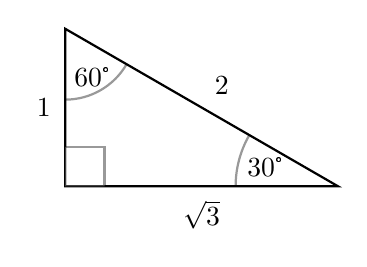
\begin{tikzpicture}[thick]
\coordinate (O) at (0,0);
\coordinate (A) at (3.4641,0);
\coordinate (B) at (0,2);
\draw (O)--(A)--(B)--cycle;
\tkzLabelSegment[below=1.5pt](O,A){\textit{$\sqrt{3}$}}
\tkzLabelSegment[left=1.5pt](O,B){\textit{$1$}}
\tkzLabelSegment[above right=1.5pt](A,B){\textit{$2$}}
\tkzMarkRightAngle[fill=white,size=0.5,opacity=.4](A,O,B)
\tkzLabelAngle[pos = 0.35](A,O,B){}
\tkzMarkAngle[fill= white,size=1.3cm,
opacity=.4](B,A,O)
\tkzLabelAngle[pos = 0.95](B,A,O){$30\degree$}
\tkzMarkAngle[fill= white,size=0.9cm,%
opacity=.4](O,B,A)
\tkzLabelAngle[pos = 0.7](O,B,A){$60\degree$}
\end{tikzpicture}
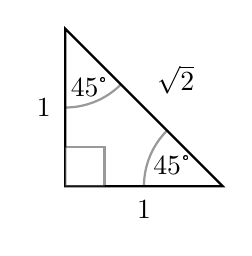
\begin{tikzpicture}[thick]
\coordinate (O) at (0,0);
\coordinate (A) at (2,0);
\coordinate (B) at (0,2);
\draw (O)--(A)--(B)--cycle;
\tkzLabelSegment[below=1.5pt](O,A){\textit{$1$}}
\tkzLabelSegment[left=1.5pt](O,B){\textit{$1$}}
\tkzLabelSegment[above right=1.5pt](A,B){\textit{$\sqrt{2}$}}
\tkzMarkRightAngle[fill=white,size=0.5,opacity=.4](A,O,B)
\tkzLabelAngle[pos = 0.35](A,O,B){}
\tkzMarkAngle[fill= white,size=1cm,%
opacity=.4](B,A,O)
\tkzLabelAngle[pos = 0.7](B,A,O){$45\degree$}
\tkzMarkAngle[fill= white,size=1cm,%
opacity=.4](O,B,A)
\tkzLabelAngle[pos = 0.8](O,B,A){$45\degree$}
\end{tikzpicture}
\end{center}

\0
\subsection{The sine rule}
	\1 Finding the sine rule

\begin{center}
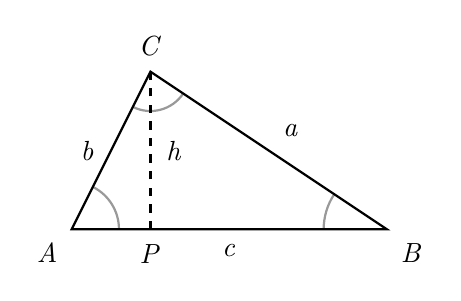
\begin{tikzpicture}[thick]
\coordinate (A) at (0,0);
\coordinate (B) at (4,0);
\coordinate (C) at (1,2);
\coordinate (P) at (1,0);
\draw (B)--(A)--(C)--cycle;
\draw [dashed] (P)--(C);

\tkzLabelSegment[below=2pt](A,B){\textit{c}}
\tkzLabelSegment[left=2pt](A,C){\textit{b}}
\tkzLabelSegment[above right=2pt](B,C){\textit{a}}
\tkzLabelSegment[right=2pt](P,C){\textit{h}}
\tkzLabelPoint[above=2pt](C){\textit{C}}
\tkzLabelPoint[below left=2pt](A){\textit{A}}
\tkzLabelPoint[below right=2pt](B){\textit{B}}
\tkzLabelPoint[below=2pt](P){\textit{P}}
\tkzMarkAngle[fill= white,size=0.6cm,%
opacity=.4](B,A,C)
\tkzMarkAngle[fill= white,size=0.5cm,%
opacity=.4](A,C,B)
\tkzMarkAngle[fill= white,size=0.8cm,%
opacity=.4](C,B,A)
\end{tikzpicture}
\end{center}
		\[\text{From }\Delta \text{CPB} \text{, } \frac{h}{a} = \text{sin } B\]
		\[\text{so\ \ \ \ \ \ \ \ } h = a \text{ sin } B\]
		\[\text{From }\Delta \text{CPA} \text{, } \frac{h}{b} = \text{sin } A\]
		\[\text{so\ \ \ \ \ \ \ \ } h = b \text{ sin } A\]
		\[\therefore a \text{ sin } B = b \text{ sin } A \text{\ \ or\ \ } \frac{a}{\text{sin } A} = \frac{b}{\text{sin } B}\]
		\[\text{Similarly:\ \ } \frac{a}{\text{sin } A} = \frac{c}{\text{sin } C} \text{\ \ and\ \ } \frac{b}{\text{sin } B} = \frac{c}{\text{sin } C}\]
		\2 When using the sine rule, label triangles with capital letters for vertices and the corresponding lower case letter for the side opposite the angle.
		\2 The sine rule states that the ratios of each side of a triangle to the sine of the opposite angle are equal. The sine rule holds true for both acute- and obtuse-angled triangles.
			\3 Equation
				\[\frac{a}{\text{sin } A} = \frac{b}{\text{sin } B} = \frac{c}{\text{sin } C}\]
		\2 The ambiguous case arises when we are given two sides and an angle that is not the included angle. Calculation of the result will yield two results: an obtuse angle, and an acute angle. There will be only one result of the equation itself, however finding the supplementary angle of the result will find the obtuse given an acute, and vice versa. The choice of using an obtuse or an acute angle is based on whether $\theta$ in the equation is obtuse or acute.
	\1 Finding a side length using the sine rule
		\2 To find an unknown side length, one must find the correct sine rule relationship to apply in the situation. Finding the unknown is as simple as substituting in values to the sine rule relationship, and solving the equation.
	\1 Finding an angle using the sine rule
		\2 

\0
\subsection{The cosine rule}

\0
\subsection{Area of a triangle}

\0
\subsection{The four quadrants}

\0
\subsection{Graphs of trigonometric functions}

\end{outline}

\newpage

\section{Quadratic equations}
\begin{outline}

\0
\subsection{Expanding expressions}
	\1 Necessary knowledge
		\2 Like terms
			\3 Like terms have the same pronumeral part. They can be collected (added and subtracted) to form a single term.
				\[7x - 11x = -4x\]
				\[4a^2b - 7ba^2 = -3a^2b\]
		\2 The distributive law
			\3 The distributive law is used to expand brackets.
				\[a(b + c) = ab + ac \text{ and } a(b - c) = ab - ac\]
				\[(a + b)(c + d) = ac + ad + bc + bd\]
	 	 	$(a + b)(c + d)$ is a binomial product because each expression within the parenthesis has two terms.
		\2 Perfect squares
	 	 	\[(a + b)^2 = (a + b)(c + d) = a^2 + 2ab + b^2\]
	 	 	\[(a - b)^2 = (a - b)(a - b) = a^2 - 2ab + b^2\]
		\2 Difference of perfect squares
	 	 	\[(a + b)(a - b) = a^2 - b^2\]
	\1 Expanding simple expressions
	\1 Expanding binomial products, perfect squares and difference of perfect squares
	\1 Expanding more binomial products

\0
\subsection{Factorising expressions}

\0
\subsection{Factorising trinomials of the form $x^2 + bx + c$}

\0
\subsection{Factorising quadratic trinomials of the form $ax^2 + bx + c$}

\0
\subsection{Factorising by completing the square}

\0
\subsection{Solving quadratic equations}

\0
\subsection{Applications of quadratics}

\0
\subsection{Solving quadratic equations by completing the square}

\0
\subsection{The quadratic formula}

\end{outline}

\newpage

\section{Measurement}
\begin{outline}

\0
\subsection{Length reiterated}
	\1 Perimeter of polygons
		\2 The perimeter of a polygon is the sum of the length of its sides, essentially being the distance around the outside of the polygon. For a simple application such as a quadrilateral, the perimeter can be found by adding together all four side lengths. When in special circumstances, such as working with a square, where all sides are equal, multiplication can be used instead of addition as a way of simplifying the equation.
			\3 Perimeter of a rectangle
				\[P = 2l + 2w = 2(l + w)\]
			\3 Perimeter of a square
				\[P = 4l\]
			\3 Perimeter of a triangle
				\[P = a + b + c\]
	\1 Circumference of a circle
		\2 The circumference (equivalent to a perimeter, but a circle has no sides) of a circle is the distance around the outside of a circle. It is found by multiplying twice the radius of the circle (essentially the diameter) with $\pi$. This is the case because of the relationship between the diameter and the circumference, where the circumference is always $\pi$ times the diameter.
			\3 There are two equations generally used to find the circumference of a circle. They are applied depending on what information is given.
				\[C = 2\pi r = \pi d\]
	\1 Perimeter of a sector
		\2 A sector is a portion of a circle, much like a slice out of a pie.
			\3 The equation to find the perimeter of a sector uses the greek letter theta, represented as $\theta$, to identify the variable angle of the sector.
				\[P = 2r+ \frac{\theta}{360} \times 2\pi r\]

\0
\subsection{Pythagoras' theorem}
	\1 Why it is used
		\2 Pythagoras' theorem is applicable only to right-angled triangles. The Pythagoras' theorem is used when one has the length of two sides of a triangle, and wants to find the third.
\begin{center}
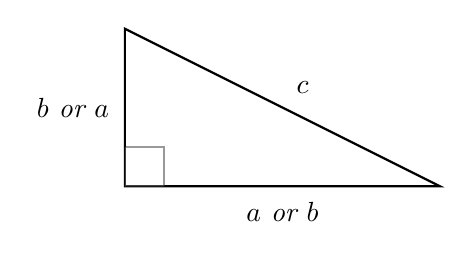
\begin{tikzpicture}[thick]
\coordinate (O) at (0,0);
\coordinate (A) at (4,0);
\coordinate (B) at (0,2);
\draw (O)--(A)--(B)--cycle;

\tkzLabelSegment[below=2pt](O,A){\textit{$a$ or $b$}}
\tkzLabelSegment[left=2pt](O,B){\textit{$b$ or $a$}}
\tkzLabelSegment[above right=2pt](A,B){\textit{$c$}}

\tkzMarkRightAngle[fill=white,size=0.5,opacity=.4](A,O,B)
\tkzLabelAngle[pos = 0.35](A,O,B){}

\end{tikzpicture}
\end{center}
	\1 Finding each side of the right-angled triangle
		\2 The longest side of the right-angled triangle is called the hypothesis. Coincidentally, the most common form of Pythagoras' theorem is for finding the hypothesis. Pythagoras' theorem can be used to find any side of a triangle, assuming one has the other two side lengths. The theorem must, however, be rearranged in order to find the other sides. For demonstrations of the Pythagoras theorem, often the letters $a$, $b$, and $c$ are used. $a$ and $b$ can be used at will, but $c$ is generally accepted to be the hypothesis.
			\3 Finding the hypothesis
				\[a^2 + b^2 = c^2\]
				\[\sqrt{a^2 + b^2} = c\]
			\3 Finding other sides
				\[c^2 - b^2 = a^2\]
				\[c^2 - a^2 = b^2\]
				\[\sqrt{c^2 - b^2} = a\]
				\[\sqrt{c^2 - a^2} = b\]

\0
\subsection{Area}
	\1 What is area?
		\2 Area is a measure of surface. As such, area is always expressed as square units, such as cm$^2$ and m$^2$. For example, a rectangle with 5 metres of width and 10 metres of length would have 50 metres squared of area.
	\1 Equations to find area
		\2 Area is usually found using a simple equation, but more complex shapes (called composite shapes) or a polygon can be separated into a number of simple equations that can be added together to find the area.
			\3 Area of a square
				\[A = l^2\]
			\3 Area of a rectangle
				\[A = lw\]
			\3 Area of a triangle
				\[A = \frac{1}{2}bh\]
			\3 Area of a rhombus/kite
				\[A = \frac{1}{2}xy\]
			\3 Area of a parallelogram
				\[A = bh\]
			\3 Area of a trapezium
				\[A = \frac{1}{2}(a+b)h\]
			\3 Area of a circle
				\[A = \pi r^2\]
			\3 Area of a sector
				\[A = \frac{\theta}{360}\pi r^2\]
	\1 Converting between units of area
		\2 To convert between units of area, one must realise that area is a squared unit, hence it is necessary to convert by $\times x^2$ or $\div x^2$ (where $x$ is 10, 100, 1000, etc.) instead of $\times x$ or $\div x$.
	\1 Using area to find unknown lengths
		\2 As the area of a polygon can be found with an equation, the equation can be rearranged to find side lengths. For example, knowing that $A = l^2$ is the equation for the area of a square, the reverse of the square operation, the square root, can be used to find the length from the area. The rearrangement of the equation would be $l = \sqrt{A}$, and is a perfectly acceptable way of finding the length of the sides within a square.

\0
\subsection{Surface area -- prisms and cylinders}
	\1 Finding the surface area of a prism
		\2 The surface area of a prism is found by adding the area of each face of the prism. In the case of, for instance, a triangular prism, there are two end faces, and the three faces created by the extrusion of the triangle.
	\1 Finding the surface area of a cylinder
		\2 The surface area of a cylinder is found by adding the area of the two circular ends to the area created by the circumference of the circles multiplied by the height of the cylinder.
			\3 Surface area of a cylinder
				\[SA = 2\pi r^2 + 2\pi rh\]

\0
\subsection{Surface area -- pyramids and cones}
	\1 Finding the surface area of a pyramid
		\2 The surface area of a pyramid is found by adding the base area of the pyramid to the area of the four triangles.
			\3 Surface area of a pyramid
				\[l^2 + 4 \times \frac{1}{2}bh\]
	\1 Finding the surface area of a cone
		\2 A cone is composed of a circle as the base, and a sector. The surface area of a cone is found by multiplying $\pi$, the radius and the slant length, then adding the area of the base.
			\3 Surface area of a cone
				\[\pi rs + \pi r^2\]

\0
\subsection{Volume -- prisms and cylinders}
	\1 Finding the volume of a prism
		\2 A prism is a polygon extended along the height axis, and as such has a uniform cross-section. The prism is named by the shape of the cross-section, hence ``triangular prism'', ``hexagonal prism'', etc. The volume of a prism is found by multiplying the area of the cross-section by the height. Thus, the formula for the volume of a prism is always the same, regardless of the cross-sectional shape.
			\3 Volume of a prism
				\[V = ah\]
	\1 Finding the volume of a cylinder
		\2 A cylinder is a circle extended along the height axis, and because of that has a perfect circle as the cross-section. The equation used to find the volume of the cylinder is the area of the circle multiplied by the height of the cylinder.
			\3 Volume of a cylinder
				\[V = ah = \pi r^2 h\]

\0
\subsection{Volume -- pyramids and cones}
	\1 Finding the volume of a pyramid
		\2 A pyramid within a cube takes up one third of the space. Therefore, the volume of a pyramid is the area of the base multiplied by the height, divided by 3.
			\3 Volume of a pyramid
				\[V = \frac{1}{3}ah\]
	\1 Finding the volume of a cone
		\2 A cone within a cube takes up one third of the space. Hence, the volume of the cone is the area of the base multiplied by the height, divided by 3.
			\3 Volume of a cone
				\[V = \frac{1}{3}ah\]

\0
\subsection{Spheres}
	\1 Finding the volume of a sphere
		\2 The volume of a sphere is calculated by multiplying the equation 4/3 by $\pi r^3$.
			\3 Volume of a sphere
				\[V = \frac{4}{3}\pi r^3\]
	\1 Finding the surface area of a sphere
		\2 The surface area of a sphere is calculated by multiplying 4 by $\pi r^2$.
			\3 Surface area of a sphere
				\[SA = 4\pi r^2\]
	\1 Finding the radius of a sphere
		\2 The radius of a sphere can be found using the volume of the sphere. Knowing the equation for volume of a sphere allows one to substitute in the known volume and solve the problem like a regular equation.

\end{outline}

\newpage

\section{Parabolas and other graphs}
\begin{outline}

\0
\subsection{Exploring parabolas}

\0
\subsection{Sketching parabolas with transformations}

\0
\subsection{Sketching $y = x^2 + bx + c$ using factorisation}

\0
\subsection{Sketching by competing the square}

\0
\subsection{Sketching using the quadratic formula}

\0
\subsection{Applications of parabolas}

\0
\subsection{Graphs of circles}

\0
\subsection{Graphs of exponentials}

\0
\subsection{Graphs of hyperbolas}

\0
\subsection{Further transformations of graphs}

\end{outline}

\newpage

\section{Probability}
\begin{outline}

\0
\subsection{Probability reiterated}
	\1 Definitions
		\2 \textbf{Trial: } A trial is a single experiment, such as a single flip of a coin.
		\2 \textbf{Sample space: } The sample space is the list of potential outcomes from an experiment.
		\2 \textbf{Outcome: } An outcome is a possible result of an experiment.
		\2 \textbf{Event: } An event is the list of favourable outcomes.
		\2 \textbf{Equally likely outcomes: } Equally likely outcomes are outcomes that have the same chance of happening.
	\1 Chance
		\2 Chance is a numerical value based on a scale from 0 to 1 that represents probability. 0 represents impossible, while 1 represents certain.
	\1 Calculating theoretical probabilities
		\2 The probability of an event in which outcomes have equal chance is calculated by dividing the number of favourable outcomes by the total number of outcomes.
			\3 Equation
				\[Pr(Event) = \frac{\text{Number of favourable outcomes}}{\text{Total number of outcomes}}\]
	\1 Calculating experimental probabilities
		\2 The probability of experiments only differ to theoretical probability in that experimental probability uses the results of an experiment, rather than relying on results that are purely theoretical with no real application. The calculation of experimental probability differs only slightly from theoretical probability in that instead of dividing the number of favourable outcomes by the total number of outcomes, it uses the total number of trials.
			\3 Equation
				\[Pr(Event) = \frac{\text{Number of favourable outcomes}}{\text{Total number of trials}}\]

\0
\subsection{Unions and intersections}
	\1 Set notation
		\2 \textbf{Set: } A set is a collection or group of elements that can include numbers, letters or other objects.
		\2 \textbf{Sample space: } The sample space, denoted by $\xi$, is the set of all possible elements or objects considered in a particular situation.
		\2 \textbf{Null set: } A null or empty set is a set with no elements and is represented by either $\varnothing$ or $\{\ \ \}$.
		\2 \textbf{Complement: } The complement is everything that isn't the event in question. The complement is represented as an $'$ after the letter, such as $A'$ compared to $A$.
		\2 \textbf{Union: } All elements that belong to either events $A$ or $B$ make up the union. A union is represented as $A\ \cup\ B$.
		\2 \textbf{Intersection: } All elements that belong to both $A$ and $B$ make up the intersection. An intersection is represented as $A\ \cap\ B$.
		\2 \textbf{Mutual exclusion: } Two sets $A$ and $B$ are mutually exclusive if they have no elements in common, meaning $A\ \cap\ B = \varnothing$.
	\1 Venn diagrams
		\2 Venn diagrams are used to illustrate how the elements in the sample space are distributed among the events.
\begin{center}
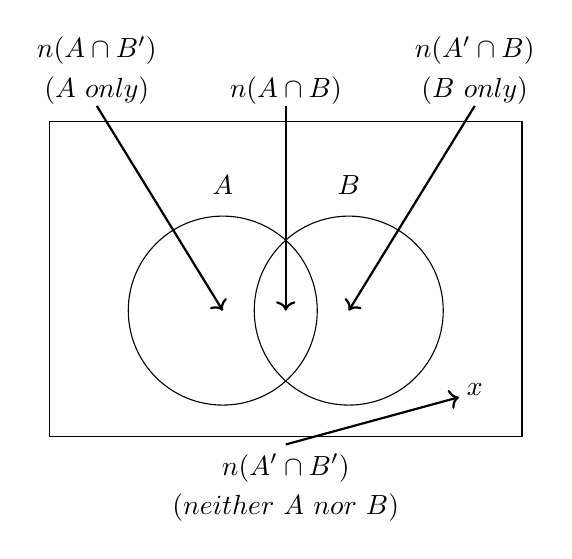
\begin{tikzpicture}[scale=2]
\draw (-1.5,-1) rectangle (1.5,1);
\draw (-0.4,-0.2) circle [radius=0.6];
\draw (0.4,-0.2) circle [radius=0.6];
\node at (-0.4,0.6) {$A$};
\node at (0.4,0.6) {$B$};
\node at (0,1.2) {$n(A \cap B)$};
\node at (-1.2,1.45) {$n(A \cap B')$};
\node at (-1.2,1.2) {$(A\ only)$};
\node at (1.2,1.45) {$n(A' \cap B)$};
\node at (1.2,1.2) {$(B\ only)$};
\node at (1.2, -0.7) {$x$};
\node at (0, -1.2) {$n(A' \cap B')$};
\node at (0, -1.45) {$(neither\ A\ nor\ B)$};
\draw[thick,->] (1.2,1.1) -- (0.4,-0.2);
\draw[thick,->] (-1.2,1.1) -- (-0.4,-0.2);
\draw[thick,->] (0,1.1) -- (0,-0.2);
\draw[thick,->] (0,-1.05) -- (1.10,-0.75);
\end{tikzpicture}
\end{center}
	\1 Listing sets
		\2 Listing sets can be useful in dealing with probability by allowing easier calculation of $Pr(Event)$ probabilities. A good way of dealing with sets is to visualise them as a Venn diagram, however everything involved can be done without visualisation. Firstly, at least in probability involving two events, it is necessary to identify the elements common to both events. With that one can find $A \cup B$, which allows $A' \cap B'$ (the elements outside event $A$ and $B$) to be found.
			\3 Example
\begin{center}
				\[\text{$A$ and $B$ involve numbers taken from integers 1:10}\]
\end{center}
				\[A = \{1,2,3,4,5,6\}\]
				\[B = \{1,3,7,8\}\]
				\[A \cap B = \{1,3\}\]
				\[A \cup B = \{1,2,3,4,5,6,7,8\}\]
				\[A' \cap B' = \{9,10\}\]
	\1 Two-way tables
		\2 Two-way tables are useful tools for organising probability data. They allow for easy mental extrapolation of all probability data when starting with little information.
\begin{center}
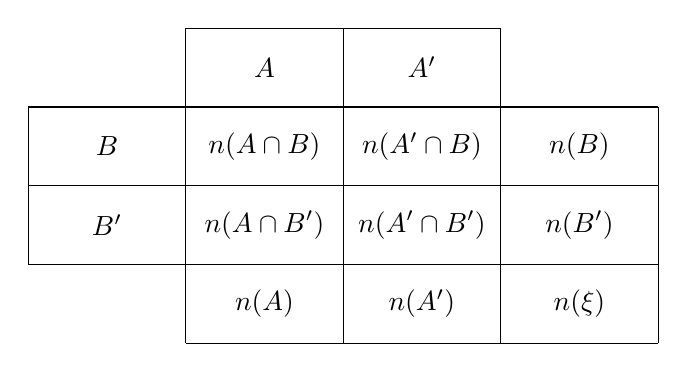
\begin{tikzpicture}[scale=0.5]
\draw (4,0) -- (12,0);
\draw (0,-2) -- (16,-2);
\draw (0,-4) -- (16,-4);
\draw (0,-6) -- (16,-6);
\draw (4,-8) -- (16,-8);
\draw (0,-2) -- (0,-6);
\draw (4,0) -- (4,-8);
\draw (8,0) -- (8,-8);
\draw (12,0) -- (12,-8);
\draw (16,-2) -- (16,-8);
\node at (6,-1) {$A$};
\node at (10,-1) {$A'$};
\node at (2,-3) {$B$};
\node at (6,-3) {$n(A \cap B)$};
\node at (10,-3) {$n(A' \cap B)$};
\node at (14,-3) {$n(B)$};
\node at (6,-5) {$n(A \cap B')$};
\node at (10,-5) {$n(A' \cap B')$};
\node at (14,-5) {$n(B')$};
\node at (2,-5) {$B'$};
\node at (6,-7) {$n(A)$};
\node at (10,-7) {$n(A')$};
\node at (14,-7) {$n(\xi)$};
\end{tikzpicture}
\end{center}	

\0
\subsection{The addition rule}
	\1 The addition rule states that the probability of $A \cap B$ taken away from $A$ added to the probability of $B$ is the same as $A \cup B$. The removal of $A \cap B$ is necessary as $A$ and $B$ both contain $A \cap B$, so subtraction is essential to avoid duplication of $A \cap B$.
	\1 Equation
		\[Pr(A \cup B) = Pr(A) + Pr(B) - Pr(A \cap B)\]
	\1 If A and B are mutually exclusive then:
		\[Pr(A \cap B) = 0\]
		\[Pr(A \cup B) = Pr(A) + Pr(B)\]

\0
\subsection{Conditional probability}
	\1 What is conditional probability
		\2 Conditional probability is probability that an event occurs given that another event has already occurred. The probability of event A occurring given that event B has occurred is denoted by $Pr(A|B)$. $Pr(A|B)$ is read as `the probability of A given B'.
			\3 Equation
				\[Pr(A|B) = \frac{Pr(A \cap B)}{Pr(B)}\ and\ Pr(B|A) = \frac{Pr(A \cap B)}{Pr(A)}\]

\0
\subsection{Multiple events using tables}
	\1 Tables with and without replacement
		\2 Replacement means outcomes can be repeated.
		
\begin{center}
Two selections are made from the digits \{1, 2, 3\}:
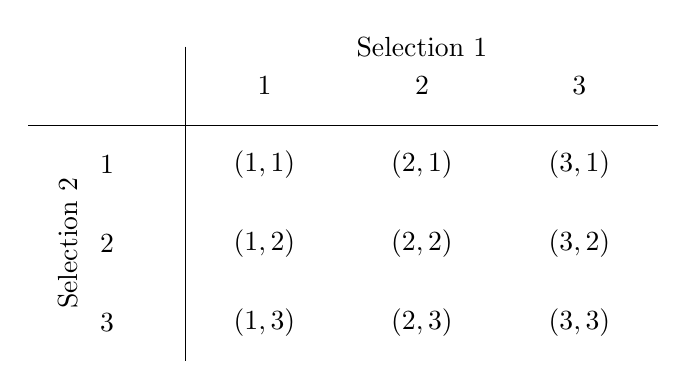
\begin{tikzpicture}[scale=0.5]
\draw (4, 0)--(4,-8);
\draw (0, -2)--(16,-2);
\node at (10,0){Selection $1$};
\node at (1,-5)[rotate=90]{Selection $2$};
\node at (6,-1){$1$};
\node at (10,-1){$2$};
\node at (14,-1){$3$};
\node at (2,-3){$1$};
\node at (2,-5){$2$};
\node at (2,-7){$3$};
\node at (6,-3){$(1,1)$};
\node at (10,-3){$(2,1)$};
\node at (14,-3){$(3,1)$};
\node at (6,-5){$(1,2)$};
\node at (10,-5){$(2,2)$};
\node at (14,-5){$(3,2)$};
\node at (6,-7){$(1,3)$};
\node at (10,-7){$(2,3)$};
\node at (14,-7){$(3,3)$};
\end{tikzpicture}
\end{center}

		\2 No replacement means that outcomes cannot be repeated. Every instance where the same event happens twice, such as $(1,1)$, $(2,2)$, and so on, must be crossed out, or otherwise notated to be an impossibility on the table, as they cannot happen.
		
\begin{center}
Two selections are made from the digits \{1, 2, 3\}:
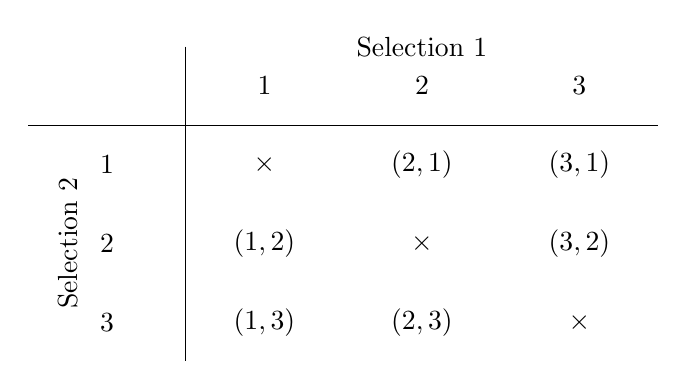
\begin{tikzpicture}[scale=0.5]
\draw (4, 0)--(4,-8);
\draw (0, -2)--(16,-2);
\node at (10,0){Selection $1$};
\node at (1,-5) [rotate=90] {Selection $2$};
\node at (6,-1){$1$};
\node at (10,-1){$2$};
\node at (14,-1){$3$};
\node at (2,-3){$1$};
\node at (2,-5){$2$};
\node at (2,-7){$3$};
\node at (6,-3){$ \times $};
\node at (10,-3){$(2,1)$};
\node at (14,-3){$(3,1)$};
\node at (6,-5){$(1,2)$};
\node at (10,-5){$ \times $};
\node at (14,-5){$(3,2)$};
\node at (6,-7){$(1,3)$};
\node at (10,-7){$(2,3)$};
\node at (14,-7){$ \times $};
\end{tikzpicture}
\end{center}

\0
\subsection{Using tree diagrams}
	\1 Applications
		\2 Tree diagrams can be used to list sample spaces for experiments involving two or more components. Branches can be used to describe the chance of the outcome at each step, and can be used to identify whether an experiment takes into account replacement or no replacement. Probability for the final outcomes may be obtained by multiplying the branch probabilities.
			\3 With replacement

\begin{center}
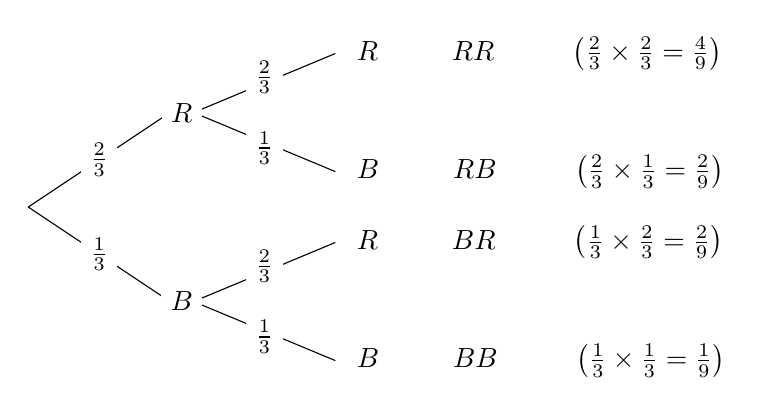
\begin{tikzpicture}[scale=0.3]
\draw (0,0)--(6,4);
\node at (3,2) [fill=white] {$\frac{2}{3}$};
\draw (7,4)--(13,6.5);
\node at (10,5.5) [fill=white] {$\frac{2}{3}$};
\draw (7,4)--(13,1.5);
\node at (10,2.5) [fill=white] {$\frac{1}{3}$};
\draw (0,0)--(6,-4);
\node at (3,-2) [fill=white] {$\frac{1}{3}$};
\draw (7,-4)--(13,-1.5);
\node at (10,-2.5) [fill=white] {$\frac{2}{3}$};
\draw (7,-4)--(13,-6.5);
\node at (10,-5.5) [fill=white] {$\frac{1}{3}$};
\node at (6.5,4) [fill=white] {$R$};
\node at (6.5,-4) [fill=white] {$B$};
\node at (13.5,6.5)[anchor=west]{$R\ \ \ \ \ \ \ \ RR\ \ \ \ \ \ \ \ \left(\frac{2}{3}\times\frac{2}{3} = \frac{4}{9}\right)$};
\node at (13.5,1.5)[anchor=west]{$B\ \ \ \ \ \ \ \ RB\ \ \ \ \ \ \ \ \left(\frac{2}{3}\times\frac{1}{3} = \frac{2}{9}\right)$};
\node at (13.5,-1.5)[anchor=west]{$R\ \ \ \ \ \ \ \ BR\ \ \ \ \ \ \ \ \left(\frac{1}{3}\times\frac{2}{3} = \frac{2}{9}\right)$};
\node at (13.5,-6.5)[anchor=west]{$B\ \ \ \ \ \ \ \ BB\ \ \ \ \ \ \ \ \left(\frac{1}{3}\times\frac{1}{3} = \frac{1}{9}\right)$};
\end{tikzpicture}
\end{center}
			\3 Without replacement
\begin{center}
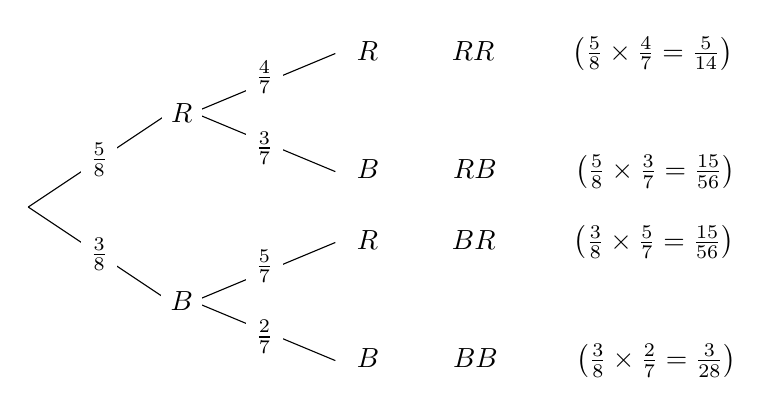
\begin{tikzpicture}[scale=0.3]
\draw (0,0)--(6,4);
\node at (3,2) [fill=white] {$\frac{5}{8}$};
\draw (7,4)--(13,6.5);
\node at (10,5.5) [fill=white] {$\frac{4}{7}$};
\draw (7,4)--(13,1.5);
\node at (10,2.5) [fill=white] {$\frac{3}{7}$};
\draw (0,0)--(6,-4);
\node at (3,-2) [fill=white] {$\frac{3}{8}$};
\draw (7,-4)--(13,-1.5);
\node at (10,-2.5) [fill=white] {$\frac{5}{7}$};
\draw (7,-4)--(13,-6.5);
\node at (10,-5.5) [fill=white] {$\frac{2}{7}$};
\node at (6.5,4) [fill=white] {$R$};
\node at (6.5,-4) [fill=white] {$B$};
\node at (13.5,6.5)[anchor=west]{$R\ \ \ \ \ \ \ \ RR\ \ \ \ \ \ \ \ \left(\frac{5}{8}\times\frac{4}{7} = \frac{5}{14}\right)$};
\node at (13.5,1.5)[anchor=west]{$B\ \ \ \ \ \ \ \ RB\ \ \ \ \ \ \ \ \left(\frac{5}{8}\times\frac{3}{7} = \frac{15}{56}\right)$};
\node at (13.5,-1.5)[anchor=west]{$R\ \ \ \ \ \ \ \ BR\ \ \ \ \ \ \ \ \left(\frac{3}{8}\times\frac{5}{7} = \frac{15}{56}\right)$};
\node at (13.5,-6.5)[anchor=west]{$B\ \ \ \ \ \ \ \ BB\ \ \ \ \ \ \ \ \left(\frac{3}{8}\times\frac{2}{7} = \frac{3}{28}\right)$};
\end{tikzpicture}
\end{center}

\0
\subsection{Independent events}
	\1 Definition
		\2 Two events are independent if the outcome of one event does not change the probability of obtaining the other event. There are two equations to check the independency of $A$ regarding $B$ or $B$ regarding $A$
			\3 Equation
				\[Pr(A | B) = Pr(A) \text{\ \ \ \ OR\ \ \ \ } Pr(B | A) = Pr(B)\]
				\[Pr(A \cap B) = Pr(A) \times Pr(B)\]
		\2 For multiple events with selection made with replacement, events are independent. For multiple events with selection made without replacement, events are not independent.

\end{outline}

\newpage

\section{Statistics}
\begin{outline}

\0
\subsection{Statistical graphs reiterated}

\0
\subsection{Quartiles}

\0
\subsection{Boxplots}

\0
\subsection{Time series data}

\0
\subsection{Bivariate data and scatter plots}

\0
\subsection{Line of best fit by eye}

\0
\subsection{Standard deviation}

\0
\subsection{Linear regression}

\end{outline}

\newpage

\section{Logarithms and polynomials}
\begin{outline}

\0
\subsection{Logarithms}

\0
\subsection{Logarithm laws}

\0
\subsection{Exponential equations using logarithms}

\0
\subsection{Polynomials}

\0
\subsection{Expanding and simplifying polynomials}

\0
\subsection{Division of polynomials}

\0
\subsection{The remainder and factor theorems}

\0
\subsection{Solving polynomial equations}

\0
\subsection{Graphs of polynomials}

\end{outline}

\newpage

\end{document}
